\section{Measure Theory I --- Measurability of Sets}
\label{sect:set-measurability}
\begin{enumerate}
\item A thorough and rigorous study of probability theory \emph{requires}
measure theory. While you may have learnt probability without ever using
measure theory before (typically the case for a first course in probability),
many concepts and terminologies you have seen are in fact measure theoretic.
For example, an \emph{event} is a \emph{measurable} set, and a \emph{random
variable} is a \emph{measurable} function. For now, you may not find the need
of introducing measure theory in the study of probability. But as we shall see,
there are indeed some pathological situations that have to be handled via
measure theory.

\item As you know from your first course in probability, \emph{events} are
sets, so let us study/review some preliminary concepts in set theory that will
be helpful for developing measure theoretic probability theory.
\end{enumerate}
\subsection{Set Theory Preliminaries}
\begin{enumerate}
\item Informally, a \emph{set} can be seen as a collection of distinct objects
or \emph{elements}.\footnote{Sometimes the terms ``set'', ``collection'', and
``family'' are used interchangeably.} While it appears to be intuitive that
such collection can be arbitrary and unrestricted, some paradoxes can actually
result if no restriction is imposed, e.g., Russell's paradox. Such issues lead
to the development of \emph{Zermelo-Fraenkel} (ZF) set theory, which imposes a
series of axioms that restrict what such ``collection'' can be.\footnote{Here
we shall not delve into the details. If you are interested, you can take a look
at
\href{https://en.wikipedia.org/wiki/Zermelo\%E2\%80\%93Fraenkel_set_theory}{its
Wikipedia page}.}

On top of the axioms in the ZF set theory, another commonly imposed axiom is
the \emph{axiom of choice}, which suggests that for all collections
\(\mathcal{A}\) of non-empty sets, there is a \emph{choice function} \(f\) such
that \(f(A)\in A\) for all \(A\in\mathcal{A}\). Intuitively, this axiom means
that it is possible to ``choose''/``pick'' an element from each set in any
fixed collection (finite or countably infinite or even uncountably infinite).

The ZF set theory together with the axiom of choice is abbreviated as
\emph{ZFC}, and we shall always work with ZFC (which is typically the case when
you encounter any mathematics involving sets).

\item \textbf{Set terminologies.} In the following, we will review
some terminologies about sets, which should be very familiar to you. Here, we
let \(\Omega\) be a nonempty \emph{universal} set (meaning that every set below
is a \emph{subset} of it).
\begin{center}
\begin{tabular}{lll}
\toprule
Name&Notation&Definition \\
\midrule
\makecell[l]{\(A\) is a subset of \(\Omega\), or \\
\(\Omega\) is a superset of \(A\)
}&
\makecell[l]{\(A\subseteq \Omega\), or \\
\(\Omega\supseteq A\)
}
&For any \(\omega\in A\), we have \(\omega\in\Omega\).  \\
\midrule
(Absolute) complement&\(A^c\)&\(\{\omega\in\Omega:\omega\notin A\}\) \\
Set difference&\(A\setminus B\)&\(A\cap B^c\) \\
Intersection (\(I\): index set)&\(\bigcap_{i\in I}A_i\)&\(\{\omega\in\Omega:\omega\in A_i\text{ for all \(i\in I\)}\}\) \\
Union &\(\bigcup_{i\in I}A_i\)&\(\{\omega\in\Omega:\omega\in A_i\text{ for some \(i\in I\)}\}\) \\
\midrule
Disjoint union &\(\biguplus_{i\in I}A_i\)&\makecell[l]{ meaning the same as \(\bigcup_{i\in I}A_i\),\\
 with the emphasis on the pairwise disjointness, \\
i.e., \(A_{i}\cap A_{j}=\varnothing\) for all \(i,j\in
I\) with \(i\ne j\).
}
 \\
\bottomrule
\end{tabular}
\end{center}
\begin{note}
The concept of complement depends on what the universal set is. In some
occasions, we may use the somewhat awkward notation \(A^{c_{\Omega}}\) to
stress that the universal set being considered is \(\Omega\) for this
complement.
\end{note}
\item \textbf{Basic set properties.} You should be very familiar to the
following properties of sets (the sets below are arbitrary):
\begin{itemize}
\item \emph{Associativity of union and intersection:} \((A\cup B)\cup C=A\cup
(B\cup C)\) and \((A\cap B)\cap C=A\cap (B\cap C)\).
\item \emph{Commutativity of union and intersection:} \(A\cup B=B\cup A\) 
and \(A\cap B=B\cap A\).
\item \emph{De Morgan's laws:} \((\bigcup_{i\in I}A_i)^{c}=\bigcap_{i\in I}A_i^{c}\)
and \((\bigcap_{i\in I}A_i)^{c}=\bigcup_{i\in I}A_i^{c}\). More generally, for
any \(B\subseteq \Omega\), we have
\(B\setminus \bigcup_{i\in I}A_i=\bigcap_{i\in I}B\setminus A_i\)
and \(B\setminus \bigcap_{i\in I}A_i=\bigcup_{i\in I}B\setminus A_i\).
\end{itemize}
Make sure you are able to \emph{prove} these! (An useful way to prove a set
equality \(S=T\) is to prove (i) \(S\subseteq T\) and (ii) \(T\subseteq S\).)

\item\label{it:further-set-term} \textbf{Further set terminologies.} For the
following set theoretic terminologies, you may not have encountered them
before, so perhaps you should pay more attention here:
\begin{center}
\begin{tabular}{lll}
\toprule
Name&Notation&Definition \\
\midrule
\defn{Infimum (set)}&\(\inf_{k\ge n}A_k\)&\(\bigcap_{k\ge n}A_k\)\\
\defn{Supremum (set)}&\(\sup_{k\ge n}A_k\)&\(\bigcup_{k\ge n}A_k\) \\
\defn{Limit inferior (set)}&\(\liminf_{n\to\infty}A_n\)&\(\bigcup_{n=1}^{\infty}\bigcap_{k\ge n}A_k
=\sup_{n\ge 1}\inf_{k\ge n}A_k\)\\
\defn{Limit superior (set)}&\(\limsup_{n\to \infty}A_n\)&\(\bigcap_{n=1}^{\infty}\bigcup_{k\ge n}A_k
=\inf_{n\ge 1}\sup_{k\ge n}A_k\) \\
\defn{Limit of \(A_n\)}&\(\lim_{n\to \infty}A_n=A\) or \(A_n\to A\)&
\(\liminf_{n\to \infty}A_n=\limsup_{n\to\infty}A_n=A\) \\
\(\{A_n\}_{n\in\N}\) is \defn{increasing}&\(A_n\nearrow\)&\(A_1\subseteq A_2\subseteq\dotsb\) \\
\(\{A_n\}_{n\in\N}\) is \defn{decreasing}&\(A_n\searrow\)&\(A_1\supseteq A_2\supseteq\dotsb\) \\
\bottomrule
\end{tabular}
\end{center}
\item \textbf{Further set properties.} Here we will discuss some results about
the less familiar set terminologies from \labelcref{it:further-set-term}:
\begin{enumerate}
\item \label{it:liminfsup-interpret} \emph{(Interpreting limit inferior and limit superior)}
\begin{enumerate}
\item \(\liminf_{n\to \infty}A_n=\{\omega\in\Omega:\omega\in A_n\text{ for
\underline{a}ll \underline{b}ut \underline{f}initely \underline{m}any \(n\)}\}
=:\{\omega\in A_n\text{ abfm}\}\).
\item
\(\limsup_{n\to \infty}A_n=\{\omega\in\Omega:\omega\in A_n\text{ for infinitely many \(n\)}\}
=\{\omega\in\Omega:\omega\in A_n\text{ \underline{i}nfinitely \underline{o}ften}\}
=:\{\omega\in A_n\text{ io}\}\).
\end{enumerate}
\begin{pf}
\begin{enumerate}
\item Note that
\[
\liminf_{n\to \infty}A_n=\bigcup_{n=1}^{\infty}\bigcap_{k\ge n}A_k
=\{\omega\in\Omega:\exists n\in\N\text{ s.t. }\omega\in A_k\;\forall k\ge n\}
\]
and ``\(\exists n\in\N\text{ s.t. }\omega\in A_k\;\forall k\ge n\)'' just means
``\(\omega\in A_n\) for all but finitely many \(n\)'' in words.

\item Similar to above, and we can interpret ``\(\forall n\in\N\; \exists k\ge
n\text{ s.t. }\omega\in A_k\)'' as ``\(\omega\in A_n\) for infinitely many \(n\)''.
\end{enumerate}
\end{pf}
\item \label{it:liminfsup-relate} \emph{(Relating limit inferior and limit superior)}
\begin{enumerate}
\item \(\liminf_{n\to \infty}A_n\subseteq \limsup_{n\to \infty}A_n \).
\item \((\liminf_{n\to \infty}A_n)^{c}=\limsup_{n\to \infty}A_n^c \).
\item \((\limsup_{n\to \infty}A_n)^{c}=\liminf_{n\to \infty}A_n^c \).
\end{enumerate}
\begin{pf}
\begin{enumerate}
\item Because ``\(\omega\in A_n\) for all but finitely many \(n\)'' is just a
special case of ``\(\omega\in A_n\) for infinitely many \(n\)''.
\item Apply De Morgan's laws twice:
\[
\left(\liminf_{n\to \infty}A_n\right)^{c}
=\left(\bigcup_{n=1}^{\infty}\vc{\bigcap_{k\ge n}A_k}\right)^{c}
\overset{\text{DM}}{=} \bigcap_{n=1}^{\infty}\vc{\left(\bigcap_{k\ge n}A_k\right)^{c}}
\overset{\text{DM}}{=} \bigcap_{n=1}^{\infty}\left(\vc{\bigcup_{k\ge n}A_k^{c}}\right)
=\limsup_{n\to \infty}A_n^c .
\]
\item Again apply De Morgan's laws twice:
\[
\left(\limsup_{n\to \infty}A_n\right)^{c}
=\left(\bigcap_{n=1}^{\infty}\vc{\bigcup_{k\ge n}A_k}\right)^{c}
\overset{\text{DM}}{=} \bigcup_{n=1}^{\infty}\vc{\left(\bigcup_{k\ge n}A_k\right)^{c}}
\overset{\text{DM}}{=} \bigcup_{n=1}^{\infty}\left(\vc{\bigcap_{k\ge n}A_k^{c}}\right)
=\liminf_{n\to \infty}A_n^c .
\]
\end{enumerate}
\end{pf}
\item \label{it:lim-mono-sets} \emph{(Limits of monotone sequences of sets)}
\begin{enumerate}
\item If \(A_n\nearrow\), then \(\lim_{n\to \infty}A_n\) exists and equals \(\bigcup_{k=1}^{\infty} A_k\).

\begin{note}
Setting \(A_n:=\bigcup_{i=1}^{n}B_i\), since \(A_n\nearrow\), we can get the
intuitively appealing equality
\(\lim_{n\to\infty}\bigcup_{i=1}^{n}B_i=\bigcup_{i=1}^{\infty}B_i\), as \(\bigcup_{i=1}^{\infty}B_i
=\bigcup_{k=1}^{\infty}\left(\bigcup_{i=1}^{k}B_k\right).\)
\end{note}
\item If \(A_n\searrow\), then \(\lim_{n\to \infty}A_n\) exists and equals \(\bigcap_{k=1}^{\infty} A_k\).
\item For any collection \(\{A_n\}\subseteq\pow{\Omega}\), \(\liminf_{n\to \infty}A_n
=\lim_{n\to \infty}(\inf_{k\ge n}A_k)\) and \(\limsup_{n\to \infty}A_n
=\lim_{n\to \infty}(\sup_{k\ge n}A_k)\). \begin{note}
This explains the rationale behind the notations ``\(\liminf_{n\to
\infty}A_n\)'' and ``\(\limsup_{n\to \infty}A_n\)''.
\end{note}
\end{enumerate}
\begin{pf}
\begin{enumerate}
\item Assuming \(A_n\nearrow\), we have \vc{\(A_k\subseteq
\bigcap_{i=k}^{\infty}A_i\)}. Hence,
\[
\limsup_{n\to \infty}A_n=\bigcap_{n=1}^{\infty}\bigcup_{k=n}^{\infty}A_k
\subseteq \boxed{\bigcup_{k=1}^{\infty}\vc{A_k}}
\vc{\subseteq} \bigcup_{n=1}^{\infty}\vc{\bigcap_{i=k}^{\infty}A_i}
=\liminf_{n\to \infty}A_n
\subseteq \limsup_{n\to \infty}A_n.
\]
This forces \(\liminf_{n\to \infty}A_n=\limsup_{n\to
\infty}A_n=\bigcup_{k=1}^{\infty}A_k\), as desired.

\item Let \(B_n=A_n^c\) for every \(n\), then \(B_n\nearrow\). Applying (i), we
get
\[
\liminf_{n\to \infty}B_n
=\limsup_{n\to \infty}B_n
=\bigcup_{k=1}^{\infty}B_k.
\]
By \labelcref{it:liminfsup-relate}, we have \(\liminf_{n\to
\infty}B_n=(\limsup_{n\to \infty}A_n)^c\) and
\(\limsup_{n\to \infty}B_n=(\liminf_{n\to \infty}A_n)^c\). It then follows that
\[
\liminf_{n\to \infty}A_n=\limsup_{n\to \infty}A_n=\left(\bigcup_{k=1}^{\infty}B_k\right)^c
=\bigcap_{k=1}^{\infty}A_k^{c}.
\]
\item Note that \(\inf_{k\ge n}A_k\nearrow\) and \(\sup_{k\ge n}A_k\searrow\).
Hence,
\[
\liminf_{n\to \infty}A_n=\bigcup_{n=1}^{\infty}\bigcap_{k=n}^{\infty}A_k
=\bigcup_{n=1}^{\infty}\inf_{k\ge n}A_k
\overset{\text{(i)}}{=}\lim_{n\to \infty}\left(\inf_{k\ge n}A_k\right)
\]
and
\[
\limsup_{n\to \infty}A_n=\bigcap_{n=1}^{\infty}\bigcup_{k=n}^{\infty}A_k
=\bigcap_{n=1}^{\infty}\sup_{k\ge n}A_k
\overset{\text{(ii)}}{=}\lim_{n\to \infty}\left(\sup_{k\ge n}A_k\right).
\]
\end{enumerate}
\end{pf}

In view of \labelcref{it:lim-mono-sets}, we sometimes write \(A_n\nearrow A\)
(\(A_n\searrow A\)) to mean \(A_n\) is increasing (decreasing) and
\(\lim_{n\to\infty}A_n=A\), i.e., \(\bigcup_{k=1}^{\infty}A_k=A\)
(\(\bigcap_{k=1}^{\infty}A_k=A\)).
\end{enumerate}
\item \textbf{Equivalence relations.} Concepts related to equivalence relation
have been discussed in MATH2012; here we will go through some key points:
\begin{itemize}
\item An \emph{equivalence relation} is a relation \(\sim\) on a set \(A\) that is
(i) reflexive: \(a\sim a\), (ii) symmetric: \(a\sim b\implies b\sim a\), and
(iii) transitive: \(\text{\(a\sim b\) and \(b\sim c\)}\implies a\sim c\).
(where \(a,b,c\) are all arbitrary elements in \(A\)).
\item The \emph{equivalence class} of \(a\in A\) under an equivalence relation
\(\sim\) on \(A\) is \([a]:=\{x\in A:x\sim a\}\), i.e., the set of all elements
in \(A\) that are ``equivalent'' to \(a\) under \(\sim\).
\item Property: Two equivalence classes are either identical or disjoint, and
\([a]=[b]\) iff \(a\sim b\).
\item Property: The set of all distinct equivalence classes, \(P=\{[a]:a\in
A\}\), forms a partition of \(A\) (i.e., the classes in \(P\) are pairwise
disjoint and their union is \(A\)).
\end{itemize}
\item \textbf{Indicator functions.} You should have learnt what an indicator
function is in your first probability course. This function continues to be of
great use here, so let us review it a bit.
\begin{itemize}
\item The \emph{indicator function} of \(A\subseteq \Omega\) is given by
\[
\indic_{A}(\omega)=\begin{cases}
1&\text{if \(\omega\in A\),} \\
0&\text{otherwise.} \\
\end{cases}
\]
\item Property: \(\indic_{A}\le\indic_{B}\) (i.e.,
\(\indic_{A}(\omega)\le\indic_{B}(\omega)\) for all \(\omega\in\Omega\)) iff
\(A\subseteq B\).
\end{itemize}
\begin{note}
In some cases, we would use the notation \(\indicset{\text{statement}}\) to
denote an indicator variable that is \(1\) if the statement is true, and \(0\)
if it is not. For example, \(\indicset{x\ge 0}=\text{\(1\) if \(x\ge 0\) and
\(\indicset{x\ge 0}=0\) otherwise} \). While it has a similar notation and carries similar
meaning as the indicator function, it may not be a function of \(\omega\)
anymore; in this example, the indicator \(\indicset{x\ge 0}\) becomes a
function of \(x\).
\end{note}

Indicator function can be applied for describing \(\limsup_{n\to \infty}A_n\)
and \(\liminf_{n\to \infty}A_n\):
\[
\limsup_{n\to \infty}A_n
=\left\{\omega\in\Omega:\sum_{n=1}^{\infty}\indic_{A_n}(\omega)=\infty\right\},\quad
\liminf_{n\to \infty}A_n
=\left\{\omega\in\Omega:\sum_{n=1}^{\infty}\indic_{A_{n}^{\rc{c}}}(\omega)<\infty\right\}.
\]
This is because when \(\omega\in A_n\) infinitely often, infinitely many
\(\indic_{A_n}(\omega)\) would equal one; when \(\omega\in A_n\) for all but
finitely many \(n\), finitely many \(\indic_{A_n^{\rc{c}}}(\omega)\) would
equal one.

\item \textbf{Images and preimages.} A pair of concepts that will frequently
appear in our discussion of measure theory is \emph{image} and \emph{preimage},
which is again covered in MATH2012.

Let \(\Omega\) and \(\Omega'\) be two sets, and \(X:\Omega\to\Omega'\) be a
function.  The \emph{image} of \(A\subseteq \Omega\) under \(X\) is
\(X(A):=\{X(\omega):\omega\in A\}\), and the \emph{preimage} of \(A'\subseteq
\Omega'\) under  is \(X^{-1}(A'):=\{\omega\in\Omega:X(\omega)\in A'\}\).
\begin{center}
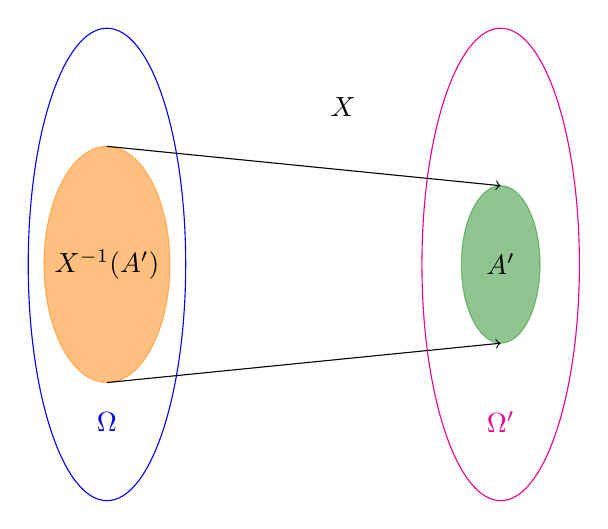
\begin{tikzpicture}
\draw[blue] (0,0) ellipse [x radius=1cm, y radius=3cm];
\draw[magenta] (5,0) ellipse [x radius=1cm, y radius=3cm];
\draw[ForestGreen, fill, opacity=0.5] (5,0) ellipse [x radius=0.5cm, y radius=1cm];
\draw[orange, fill, opacity=0.5] (0,0) ellipse [x radius=0.8cm, y radius=1.5cm];
\draw[->] (0,1.5) -- (5,1);
\draw[->] (0,-1.5) -- (5,-1);
\node[] () at (0,0) {\(X^{-1}(A')\)};
\node[] () at (5,0) {\(A'\)};
\node[] () at (3,2) {\(X\)};
\node[blue] () at (0,-2) {\(\Omega\)};
\node[magenta] () at (5,-2) {\(\Omega'\)};
\end{tikzpicture}
\end{center}
Let \(\mathcal{A}'\) be a family of sets in \(\Omega'\) (i.e., a subset of
\(\mathcal{P}(\Omega')\). Then, the notation \(X^{-1}(\mathcal{A}')\) refers to
the set of all preimages of sets in \(\mathcal{A}\), i.e.,
\(\{X^{-1}(A'):A'\in\mathcal{A}'\}\).
\item\label{it:preimg-prop} \textbf{Properties of preimages.} Let \(A'\) be any
subset of \(\Omega'\), and \(\{A_i'\}_{i\in I}\) be any collection of subsets of
\(\Omega'\).
\begin{enumerate}
\item \emph{(preservation of complementation)} \(\big(X^{-1}(A')\big)^{c}=X^{-1}(A'^{c})\).
\item \emph{(preservation of union)} \(X^{-1}(\bigcup_{i\in I}A_i')=\bigcup_{i\in I}X^{-1}(A_i')\).
\item \emph{(preservation of intersection)} \(X^{-1}(\bigcap_{i\in I}A_i')=\bigcap_{i\in I}X^{-1}(A_i')\).
\item \emph{(monotonicity)} Let \(\mathcal{A}',\mathcal{B}'\subseteq
\mathcal{P}(\Omega')\). Then, \(\mathcal{A}'\subseteq \mathcal{B}'\implies
X^{-1}(\mathcal{A}')\subseteq X^{-1}(\mathcal{B}')\).
\end{enumerate}
\begin{pf}
We demonstrate the proof for (b) and (d) here and leave the rest as exercises.

\begin{enumerate}
\item[(b)]
``\(\subseteq\)'': Fix any \(\omega\in X^{-1}(\bigcup_{i\in I}A_i')\). By
definition, \(X(\omega)\in\bigcup_{i\in I}A_i'\), thus there exists some \(i\in
I\) such that \(X(\omega)\in A_i'\), or \(\omega\in X^{-1}(A_i')\). This means
\(\omega\in \bigcup_{i\in I}X^{-1}(A_i')\).

``\(\supseteq\)'': Highly similar to ``\(\subseteq\)''; just work backward.

\item[(d)] Assume \(\mathcal{A}'\subseteq \mathcal{B}'\). Now, fix any \(A\in
X^{-1}(\mathcal{A}')\). By definition, we have \(A=X^{-1}(A')\) for some
\(A'\in\mathcal{A}'\). Since \(\mathcal{A}'\subseteq \mathcal{B}'\), we also
have \(A'\in\mathcal{B}'\), meaning that
\(A\in\{X^{-1}(A'):A'\in\mathcal{B}'\}=X^{-1}(\mathcal{B}')\).
\end{enumerate}
\end{pf}
\end{enumerate}
\subsection{Non-Measurable Sets}
\begin{enumerate}
\item A critical concept in measure theory is \emph{measurable set}. Roughly
speaking, it refers to any set whose ``volume'' (or ``length'', or ``area'', or
\emph{probability} later...) can be measured. A natural and important question
is then, are there really sets that \emph{cannot} be measured? The answer is
yes, and actually the existence of \emph{non-measurable} sets leads to many
interesting and fruitful developments in measure theory.

\item\label{it:meas-intuitive} Before discussing non-measurable sets, let us
first consider what is meant by ``measure'' intuitively\footnote{We will define
\emph{measure} more formally later.}. First, we can view a measure as a
function \(\lambda\) that assigns a value (``volume'') to a set. For
simplicity, let us focus on the case where the universal set is
\(\Omega=\R\) here.

A ``reasonable measure'' \(\lambda:\mathcal{F}\to [0,\infty]\)\footnote{The
domain \(\mathcal{F}\) is a family of sets in \(\Omega=\R\). We choose the
codomain as \([0,\infty]\) since it makes sense for a ``volume'' to be always
nonnegative, and we sometimes want to assign ``infinite volume''.} should
satisfy the following:
\begin{enumerate}[label={(\arabic*)}]
\item \emph{(assigning to an interval its length)} \(\lambda((a,b])=b-a\) for
any \(a,b\in\R\) with \(a\le b\).  Here, \((a,b]\) can be replaced by
\((a,b)\), \([a,b)\), or \([a,b]\).
\item \emph{(invariant under translation, rotations, and reflections)}
\(\lambda\) assigns the same value to \emph{congruent} sets (i.e., one can be
obtained from another using just translations, rotations, and reflections).
\item \emph{(\(\sigma\)-additivity)} Given any pairwise disjoint collection
\(\{A_i\}_{i\in\N}\subseteq\mathcal{F}\), we have
\(\lambda(\biguplus_{i=1}^{\infty}A_i)=\sum_{i=1}^{\infty}\lambda(A_i)\).

\begin{note}
While (finite) \emph{additivity} appears to be a more natural requirement
(obtained by changing \(\N\to\{1,\dotsc,n\}\) and \(\infty\to n\) above), the
``\(\sigma\)-'' part is necessary for working with limiting argument.

On the other hand, requiring \emph{uncountable} additivity would be way too
strong since in such case we would have, for all \(A\in\mathcal{F}\),
\[
\lambda(A)=\lambda\left(\bigcup_{x\in A}\{x\}\right)
\overset{\text{uncountable add.}}{=}
\sum_{x\in A}^{}\lambda(\{x\})
:=\sup_{B\subseteq A,\; B\text{ finite}}\sum_{x\in B}^{}\underbrace{\lambda(\{x\})}_{\lambda([x,x])=x-x=0}
=0,
\]
which means that \emph{every} set has a ``zero volume''!
\end{note}
\end{enumerate}
Based on these requirements, we can deduce:
\begin{enumerate}
\item \(\lambda(\varnothing)=0\).
\item \emph{(additivity)} For any \(\{A_i\}_{i=1}^{n}\subseteq\pow{\R}\), we have
\(\lambda(\biguplus_{i=1}^{n}A_i)=\sum_{i=1}^{n}\lambda(A_i)\).
\item \emph{(monotonicity)} For any \(A\subseteq B\), we have
\(\lambda(A)\le\lambda(B)\) .
\end{enumerate}
\begin{pf}
\begin{enumerate}
\item \(\lambda(\varnothing)=\lambda((a,a])=a-a=0\).
\item \(\lambda(\biguplus_{i=1}^{n}A_i)=\lambda(\biguplus_{i=1}^{n}A_i\uplus\varnothing\uplus\varnothing\uplus\dotsb)
\overset{\text{\(\sigma\)-add.}}{=}\sum_{i=1}^{n}\lambda(A_i)+\sum_{i=n+1}^{\infty}0=\sum_{i=1}^{n}\lambda(A_i)\).
\item \(\lambda(B)=\lambda(B\uplus(B\setminus A))=\lambda(A)
+\underbrace{\lambda(B\setminus A)}_{\ge 0}\ge \lambda(A)\).
\end{enumerate}
\end{pf}
\item Now we are ready to start discussing non-measurable sets. The idea is
that, if every set was measurable and there were not non-measurable sets, then
we could simply set \(\mathcal{F}\) as \(\pow{\R}\), allowing every subset of
\(\R\) to be measured by \(\lambda\) (being ``measurable'' in this sense). Now,
the issue is that, setting \(\mathcal{F}=\pow{\R}\) would actually lead to a
contradiction \warn{} as suggested by the following theorem:

\begin{theorem}[Vitali's theorem]
\label{thm:vitali}
There is \rc{no} \(\lambda\) defined on \(\pow{\R}\) satisfying (1)-(3) in
\labelcref{it:meas-intuitive}.
\end{theorem}
\begin{pf}
The proof is by explicitly constructing a set \(V\) (known as \defn{Vitali
set}) living in \(\pow{\R}\) such that for every \(\lambda\) on \(\pow{\R}\)
satisfying (a)-(c), any choice of value for \(\lambda(V)\) would lead to a
contradiction.

\textbf{Defining equivalence relation.} We start with the interval \([0,1]\)
and define an equivalence relation \(\sim\) on \([0,1]\) by \(x\sim y\) if
\(x-y\in \Q\), or in words, two values in \([0,1]\) are ``equivalent'' (under
\(\sim\)) if they have a rational difference. (Check \(\sim\) is indeed an
equivalence relation!)

\textbf{Constructing Vitali set \(V\).} Then, the \emph{Vitali set} \(V\) is
constructed by picking exactly one element from each distinct equivalence class
under \(\sim\), and collecting them together (possible under the axiom of
choice!).  Symbolically, we can write:
\[
V=\{v\in[0,1]:\forall x\in [0,1]\; \exists! v\in [x]\}.
\]
\begin{note}
Although the condition ``\(\forall x\in [0,1]\; \exists! v\in [x]\)'' does not
only consider distinct classes (it involves all possible equivalence classes
indeed), it does not matter because for identical equivalence classes, the
condition would be satisfied by the same unique element \(v\) picked.
\end{note}
\begin{center}
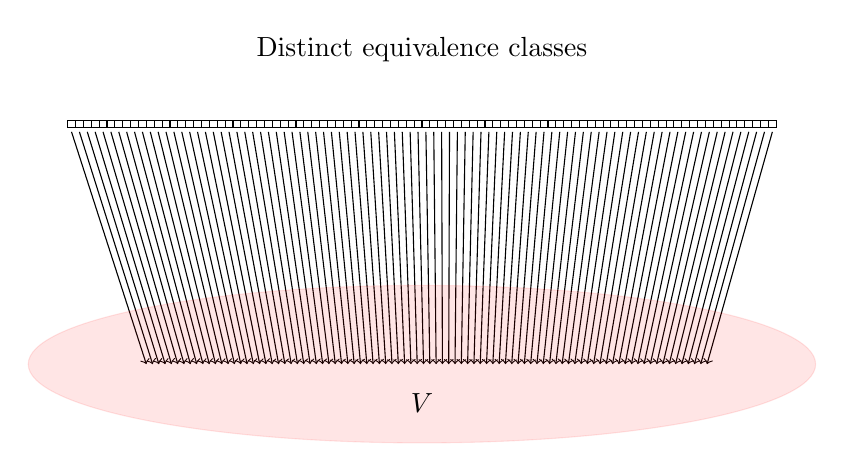
\begin{tikzpicture}
\foreach \x in {0,0.1,...,9} {
\draw[] (\x, 0) rectangle (\x+0.1, 0.1);
\draw[->] (\x+0.05, -0.05) -- (\fpeval{1+0.8*\x},-3);
}
\draw[red, fill, opacity=0.1] (4.5,-3) ellipse [x radius=5cm, y radius=1cm];
\node[] () at (4.5,-3.5) {\(V\)};
\node[] () at (4.5,1) {Distinct equivalence classes};
\end{tikzpicture}
\end{center}

\textbf{Shifting Vitali set \(V\) by rationals.}
Next, we enumerate \(\Q\cap[-1,1]\) in a \emph{diagonal} way (used for proving
the well-known result that \(\Q\) is countable) with repeated values or values
lying outside \([-1,1]\) being skipped, to form an infinite sequence
\(\{q_k\}_{k\in\N}\) of \emph{distinct} rational numbers in \([-1,1]\).

The rational numbers in \(\{q_k\}\) are then used to ``shift'' the Vitali set
\(V\) to yield \(V_k:=V+q_k:=\{v+q_k:v\in V\}\) for every \(k\in\N\).

\textbf{Proving two auxiliary claims.}

\textbf{Claim 1:} \([0,1]\subseteq \bigcup_{k=1}^{\infty}V_k\subseteq [-1,2]\).

\begin{pf}
By construction, \(V_k\subseteq [-1,2]\) for every \(k\in\N\), thus
\(\bigcup_{k=1}^{\infty}V_k\subseteq [-1,2]\). Next, fix any \(x\in [0,1]\). By
construction of \(V\), we have \(x\in [v]\) for some \(v\in V\), which means
that for some \(k\in\N\), \(x-v=q_k\) or \(x=v+q_k\in V_k\). This shows that
\([0,1]\subseteq \bigcup_{k=1}^{\infty}V_k\).
\end{pf}

\textbf{Claim 2:} \(V_k\)'s are pairwise disjoint.

\begin{pf}
Suppose not, then there is \(x\in V_k\cap V_j\) for some \(k\ne j\). Then, we
can write \(x=v_k+q_k\) and \(x=v_j+q_j\) for some \(v_k,v_j\in V\) and
\emph{distinct} \(q_k,q_j\in \Q\cap[-1,1]\). This implies that \(v_k=x-q_k\ne
x-q_j=v_j\). However, we have \(v_k-x=-q_k\in\Q\) and \(v_j-x=-q_j\in\Q\), thus
\(v_k\sim x\) and \(x\sim v_j\), which implies \(v_k\sim v_j\) by transitivity
(i.e., \(v_k\) and \(v_j\) are in the same equivalence class).  This means
\(V\) contains two \emph{distinct} elements in the \emph{same} equivalence
class, contradiction.
\end{pf}

\textbf{Showing the contradiction.}
With the two claims established, we can write \([0,1]\subseteq
\biguplus_{k=1}^{\infty}V_k\subseteq [-1,2]\). Then, by monotonicity of \(\lambda\), we have
\[
1=\lambda([0,1])\le\lambda\left(\biguplus_{k=1}^{\infty}V_k\right)\le\lambda([-1,2])=3.
\]
Applying \(\sigma\)-additivity on \(\lambda(\biguplus_{k=1}^{\infty}V_k)\) gives
\(1\le\sum_{k=1}^{\infty}\lambda(V_k)\le 3\). Note that
\(\lambda(V_k)=\lambda(V)\) by the invariance under translation, so
\(\sum_{k=1}^{\infty}\lambda(V_k)=\sum_{k=1}^{\infty}\lambda(V)\). But then
this sum is either \(0\) (when \(\lambda(V)=0\)) or \(\infty\) (when
\(\lambda(V)>0\)). Neither is between \(1\) and \(3\), contradiction.
\end{pf}

The Vitali set \(V\) in the proof is an example of \emph{non-measurable} set.
Assigning a ``volume'' to \(V\) would break the mathematics. This suggests that
the power set \(\pow{\R}\) is ``too large'' and contains some ``pathological''
sets like the Vitali set. This calls for the need to define \(\lambda\) on only
a selected collection of sets, which can be constructed using the concepts to
be introduced in \Cref{subsect:set-system}.

\item Another interesting example of non-measurable set is given by the
\emph{Banach-Tarski paradox}.
\begin{theorem}[Banach-Tarski paradox]
\label{thm:banach-tarski}
Let \(d\ge 3\) be an integer, and \(A,B\subseteq \R^d\) be any bounded sets
with nonempty interior. Then, for some \(k\in\N\), there exist pairwise
disjoint collections \(\{A_i\}_{i=1}^{k}\) and \(\{B_i\}_{i=1}^{k}\) such that
\(A=\biguplus_{i=1}^{k}A_i\) and \(B=\biguplus_{i=1}^{k}B_i\) where \(A_i\) and
\(B_i\) are congruent for every \(i=1,\dotsc,k\).
\end{theorem}
\begin{pf}
It is quite technical and hence omitted.
\end{pf}

The paradoxical feature of \Cref{thm:banach-tarski} is that while there is no
limitation on how the sizes/``volumes'' of \(A\) and \(B\) can differ, e.g.,
\(A\) can be a very small ``pea \gc{\(\bullet\)}'' and \(B\) can be the very
large ``sun \faIcon{sun}'', each of them can always be decomposed into finitely
many pieces where every pair of pieces is \emph{congruent} (``same in
size'')\warn{}.  Informally, we may say that \textit{``a pea \gc{\(\bullet\)}
can be chopped up and reassembled into the sun \faIcon{sun}''}. What went wrong
here?

The main issue is again related to non-measurable sets. We claim that at least
one set in the collections \(\{A_i\}_{i=1}^{k}\) and \(\{B_i\}_{i=1}^{k}\) is
non-measurable. Suppose not, then additivity would imply that
\(\lambda(A)=\lambda(\biguplus_{i=1}^{k}A_i)=\sum_{i=1}^{k}\lambda(A_i)
\overset{\text{invariance}}{=}\sum_{i=1}^{k}\lambda(B_i)=\lambda(\biguplus_{i=1}^{k}B_i)=\lambda(B)\).
But we can select \(A\) and \(B\) that get different assigned values by
\(\lambda\). Contradiction.
\end{enumerate}
\subsection{Systems of Sets}
\label{subsect:set-system}
\begin{enumerate}
\item \emph{Systems of sets} are utilized for constructing families of
``selected'' sets on which a ``reasonable measure'' \(\lambda\) can be defined
consistently without having any issue (those sets are \emph{measurable sets};
see \labelcref{it:meas-basic-terms} for the formal definition).  There are
multiple systems of sets here, but they all share a common theme, which is
about constructing a family \(\mathcal{A}\) of sets that is \emph{closed} under
certain set operations, i.e., performing these operations on sets in
\(\mathcal{A}\) would not yield something outside \(\mathcal{A}\) --- being
``stable'' in some sense.  Intuitively, we are interested in this kind of
properties because they can make the families of sets ``rich enough'', in the
sense that the families contain ``sufficiently many well-behaved sets''.

The systems of sets to be discussed here are: (i) semiring, (ii) ring, (iii)
algebra, and (iv) \ystar{} \(\sigma\)-algebra (important concept for
probability theory!).

\item \textbf{Definitions.}
\begin{itemize}
\item A family \(\mathcal{A}\subseteq \pow{\Omega}\) is a \defn{semiring} on
\(\Omega\) if
\begin{enumerate}[label={(\arabic*)}]
\item \(\varnothing\in\mathcal{A}\).
\item \emph{(``stable'' under set differences)}
\(A,B\in\mathcal{A}\implies A\setminus B=\biguplus_{i=1}^{n}A_i\) for
some pairwise disjoint \(A_1,\dotsc,A_n\in\mathcal{A}\), where \(n\in\N\).
\item \emph{(closed under intersections)} \(A,B\in\mathcal{A}\implies A\cap B\in\mathcal{A}\).
\end{enumerate}
\begin{note}
The ``stability'' under set differences suggests that, while taking set
differences may yield something outside \(\mathcal{A}\), we can still express
the result as a disjoint union of finitely many sets in \(\mathcal{A}\) (so
still ``stable'' to a certain degree).
\end{note}
\item A family \(\mathcal{A}\subseteq \pow{\Omega}\) is a \defn{ring} on \(\Omega\) if
\begin{enumerate}[label={(\arabic*)}]
\item \(\varnothing\in\mathcal{A}\).
\item \emph{(closed under set differences)}
\(A,B\in\mathcal{A}\implies A\setminus B\in\mathcal{A}\).
\item \emph{(closed under unions)} \(A,B\in\mathcal{A}\implies A\cup B\in\mathcal{A}\).
\end{enumerate}
\item A family \(\mathcal{A}\subseteq \pow{\Omega}\) is an \defn{algebra} (or
\defn{field}) on \(\Omega\) if
\begin{enumerate}[label={(\arabic*)}]
\item \(\varnothing\in\mathcal{A}\).
\item \emph{(closed under complementations)} \(A\in\mathcal{A}\implies A^c=\Omega\setminus A\in\mathcal{A}\).
\item \emph{(closed under unions)}
\(A,B\in\mathcal{A}\implies A\cup B\in\mathcal{A}\).
\end{enumerate}
\item \ystar{} A family \(\mathcal{A}\subseteq \pow{\Omega}\) is a
\defn{\(\sigma\)-algebra} (or \defn{\(\sigma\)-field}) on \(\Omega\) if
\begin{enumerate}[label={(\arabic*)}]
\item \(\varnothing\in\mathcal{A}\).
\item \emph{(closed under complementations)} \(A\in\mathcal{A}\implies A^c=\Omega\setminus A\in\mathcal{A}\).
\item \emph{(closed under countable unions)}
\(A_1,A_2,\dotsc\in\mathcal{A}\implies \bigcup_{i=1}^{\infty}A_i\in\mathcal{A}\).
\end{enumerate}
\begin{note}
A \(\sigma\)-algebra is actually also closed under countable
\emph{intersections}. To show this, we can use De Morgan laws, and the
closedness under countable unions and complementations:
\[
A_1,A_2,\dotsc\in\mathcal{A}
\implies \bigcap_{i=1}^{\infty}A_i\overset{\text{DM}}{=}
\left(\bigcup_{i=1}^{\infty}A_i^{c}\right)^{c}
\in\mathcal{A}.
\]
\end{note}
\end{itemize}
\item \textbf{Relationships between systems of sets.} It turns out that these
four systems are imposing stronger requirements in the order of introduction,
resulting in this chain of relationships:
\(\text{\(\sigma\)-algebra}\subsetneq\text{algebra}\subsetneq\text{ring}\subsetneq\text{semiring}\),
or in words, every \(\sigma\)-algebra is an algebra; every algebra is a ring;
etc., with the inclusion being strict, i.e., some algebra is not
\(\sigma\)-algebra; some ring is not algebra; etc.

\begin{proposition}[Relationships between systems of sets]
\label{prp:set-systems-relate}
\hfill
\begin{enumerate}
\item \(\text{\(\sigma\)-algebra}\subsetneq\text{algebra}\subsetneq\text{ring}\subsetneq\text{semiring}\).
\item An algebra on a \emph{finite} set \(\Omega\) is a \(\sigma\)-algebra.
\item A semiring that is also closed under unions is a ring.
\end{enumerate}
\end{proposition}
\begin{pf}
\begin{enumerate}
\item 
\begin{itemize}
\item \underline{\(\text{\(\sigma\)-algebra}\subsetneq \text{algebra}\)} \\
\textbf{Inclusion:} Fix any \(\sigma\)-algebra \(\mathcal{A}\) on \(\Omega\),
and any \(A,B\in\mathcal{A}\). Let \(A_1=A\), \(A_2=B\), and
\(A_3=A_4=\dotsb=\varnothing\). Applying closedness under countable unions, we get
\(A\cup B=\bigcup_{i=1}^{\infty}A_i\in\mathcal{A}\). This means \(\mathcal{A}\)
is closed under unions, thus is an algebra.

\textbf{Strictness:} Take \(\Omega=(0,1]\) and
\(\mathcal{A}=\{\biguplus_{i=1}^{n}(a_i,b_i]: 0\le a_i\le b_i\le 1, n\in\N\}\)
(or in words, the family of all possible finite disjoint unions of intervals of
the form \((a,b]\) (i.e., left-open and right-closed intervals) lying in
\(\Omega=(0,1]\)).

It can be directly checked that \(\mathcal{A}\) is an algebra.
\begin{center}
\begin{tikzpicture}
\draw[-Latex] (0,0) -- (10,0);
\node[blue] () at (2,0) {(};
\node[blue] () at (8,0) {]};
\node[blue] () at (5,0.5) {\(\Omega\)};
\node[magenta] () at (4,0) {(};
\node[magenta] () at (5,0) {]};
\node[] () at (4,-0.5) {\(a_1\)};
\node[] () at (5,-0.5) {\(b_1\)};
\node[magenta] () at (5.5,0) {(};
\node[magenta] () at (7.5,0) {]};
\node[] () at (5.5,-0.5) {\(a_2\)};
\node[] () at (7.5,-0.5) {\(b_2\)};
\draw[magenta] (4.5,-0.2) -- (6,-1);
\draw[magenta] (6.5,-0.2) -- (6,-1);
\node[] () at (6,-1.3) {\((a_1,b_1]\uplus(a_2,b_2]\)};
\draw[line width=0.2cm, magenta, opacity=0.2] (4,0) -- (5,0);
\draw[line width=0.2cm, magenta, opacity=0.2] (5.5,0) -- (7.5,0);
\end{tikzpicture}
\begin{tikzpicture}
\draw[-Latex] (0,0) -- (10,0);
\node[blue] () at (2,0) {(};
\node[blue] () at (8,0) {]};
\node[blue] () at (5,0.5) {\(\Omega\)};
\node[ForestGreen] () at (4,0) {]};
\node[ForestGreen] () at (5,0) {(};
\node[ForestGreen] () at (5.5,0) {]};
\node[ForestGreen] () at (7.5,0) {(};
\draw[ForestGreen] (3,-0.2) -- (6,-1);
\draw[ForestGreen] (5.25,-0.2) -- (6,-1);
\draw[ForestGreen] (7.75,-0.2) -- (6,-1);
\node[] () at (6,-1.3) {\(\big((a_1,b_1]\uplus(a_2,b_2]\big)^{c}\)};
\draw[line width=0.2cm, ForestGreen, opacity=0.2] (2,0) -- (4,0);
\draw[line width=0.2cm, ForestGreen, opacity=0.2] (5,0) -- (5.5,0);
\draw[line width=0.2cm, ForestGreen, opacity=0.2] (7.5,0) -- (8,0);
\end{tikzpicture}
\end{center}
However, \(\mathcal{A}\) is not a \(\sigma\)-algebra because we have
\((0,1)=\bigcup_{n=1}^{\infty}(0,1-1/n]\) with \((0,1-1/n]\in\mathcal{A}\) for
every \(n\), but \((0,1)\notin \mathcal{A}\) as finite disjoint union of
left-open and right-closed intervals must still be left-open and right-closed.
\item \underline{\(\text{algebra}\subsetneq\text{ring}\)} \\
\textbf{Inclusion:} Fix any algebra \(\mathcal{A}\) on \(\Omega\), and any
\(A,B\in\mathcal{A}\).  Applying closedness under complementations and unions,
we have \(A\setminus B=A\cap B^c\overset{\text{DM}}{=}(A^c\cup B)^c\in\mathcal{A}\).
This shows \(\mathcal{A}\) is closed under set differences, and hence is a
ring.

\textbf{Strictness:} Take \(\Omega=\{1\}\) and \(\mathcal{A}=\{\varnothing\}\).
It is not hard to see that \(\mathcal{A}\) is a ring, but \(\mathcal{A}\) is
not an algebra since \(\varnothing^c=\Omega=\{1\}\notin \mathcal{A}\).

\item \underline{\(\text{ring}\subsetneq\text{semiring}\)} \\
\textbf{Inclusion:} Fix any ring \(\mathcal{A}\) on \(\Omega\), and any \(A,B\in\mathcal{A}\).
Applying closedness under set differences, we get
\(A\cap \vc{B}\overset{\text{DM}}{=}A\cap\vc{(A\cap B^c)^c}
=A\setminus (A\setminus B)\in \mathcal{A}\), and also
\(A\setminus B=\underbrace{(A\setminus B)}_{\in\mathcal{A}}\uplus\underbrace{\varnothing}_{\in \mathcal{A}}\).

\textbf{Strictness:} Take \(\Omega=\{1,2\}\) and \(\mathcal{A}=\{\varnothing,\{1\},\{2\}\}\).
It is straightforward to check that \(\mathcal{A}\) is a semiring, but
\(\mathcal{A}\) is not a ring as \(\{1\}\cup\{2\}=\{1,2\}\notin\mathcal{A}\).
\end{itemize}
\item Because every countably infinite union of sets in \(\mathcal{A}\) can
always be expressed as a finite union of sets in \(\mathcal{A}\) in such case,
by removing redundancies.
\item Assuming a semiring \(\mathcal{A}\) is closed under unions, by induction
we have \(A_1,\dotsc,A_n\in\mathcal{A}\implies
\bigcup_{i=1}^{n}A_i\in\mathcal{A}\) for all \(n\in\N\). By the
``stability'' under set differences we have \(A,B\in\mathcal{A}\implies
A\setminus B=\biguplus_{i=1}^{n}A_i\), where \(A_1,\dotsc,A_n\in\mathcal{A}\)
are pairwise disjoint. But then by the closedness under union, we have
\(\biguplus_{i=1}^{n}A_i\in\mathcal{A}\). Thus, \(\mathcal{A}\) is closed under
set differences, hence is a ring.
\end{enumerate}
\end{pf}
\item Due to the importance of \(\sigma\)-algebra in probability theory, let us
try to understand it better through some examples in the following.
We start with the two simplest ones:
\begin{itemize}
\item The \defn{trivial \(\sigma\)-algebra} on \(\Omega\) is
\(\mathcal{F}=\{\varnothing,\Omega\}\).
\begin{note}
It is the \emph{smallest} \(\sigma\)-algebra on \(\Omega\), i.e., every
\(\sigma\)-algebra on \(\Omega\) is a superset of the trivial
\(\sigma\)-algebra.  This is because containing \(\varnothing\) and being
closed under complementations would force a \(\sigma\)-algebra to at least
contain \(\varnothing\) and \(\Omega\).
\end{note}
\item The power set \(\mathcal{F}=\mathcal{P}(\Omega)\) is a \(\sigma\)-algebra
on \(\Omega\).

\begin{remark}
\item It is a \(\sigma\)-algebra on \(\Omega\) because complement of subset of \(\Omega\) is still a subset of \(\Omega\), and countable union of subsets of \(\Omega\) is still a subset of \(\Omega\).
\item It is the \emph{largest} \(\sigma\)-algebra on \(\Omega\), i.e., every
\(\sigma\)-algebra on \(\Omega\) is a subset of \(\mathcal{P}(\Omega)\) (which
follows from definition).
\end{remark}
\end{itemize}

\item\label{it:construct-sig-alg-one} \textbf{Constructing a \(\sigma\)-algebra from one set.} Start with a set
\(A\subseteq \Omega\). Then consider the following two sets that partition
\(\Omega\):
\[
A\qquad A^c
\]
By putting zero/one/two of them into an union, we can get 4 combinations:
\begin{itemize}
\item \emph{zero:} \(\varnothing\)
\item \emph{one:} \(A\), \(A^c\)
\item \emph{two:} \(A\cup A^c=\Omega\)
\end{itemize}
These four sets form a \(\sigma\)-algebra: \(\{\varnothing, A, A^c, \Omega\}\).

\item\label{it:construct-sig-alg-two} \textbf{Constructing a \(\sigma\)-algebra
from two sets.} Here we start with two sets \(A,B\subseteq \Omega\), where
\(A\not\subseteq B\), \(B\not\subseteq A\), \(A\cap B\ne\varnothing\), and
\(A\cup B\ne\Omega\).  (These conditions are for ensuring the
\(\sigma\)-algebra constructed below has no repeated members.)

Then consider the following \(2^2=4\) sets that partition \(\Omega\): \(A\cap
B\), \(A^c\cap B\), \(A\cap B^c\), and \(A^c\cap B^c\).
\begin{center}
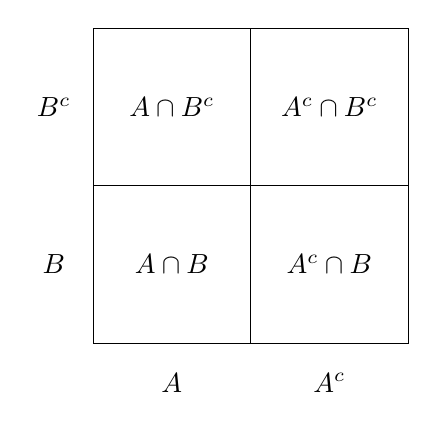
\begin{tikzpicture}
\draw[] (0,0) rectangle (2,2);
\draw[] (0,4) rectangle (2,2);
\draw[] (4,0) rectangle (2,2);
\draw[] (2,2) rectangle (4,4);
\node[] () at (1,-0.5) {\(A\)};
\node[] () at (3,-0.5) {\(A^c\)};
\node[] () at (-0.5,1) {\(B\)};
\node[] () at (-0.5,3) {\(B^{c}\)};
\node[] () at (1,1) {\(A\cap B\)};
\node[] () at (3,1) {\(A^c\cap B\)};
\node[] () at (1,3) {\(A\cap B^c\)};
\node[] () at (3,3) {\(A^c\cap B^c\)};
\end{tikzpicture}
\end{center}
By putting zero/one/two/three/four of them into an union, we can get \(\binom{4}{0}+\binom{4}{1}+\binom{4}{2}+\binom{4}{3}+\binom{4}{4}=(1+1)^4=16\) combinations:
\begin{itemize}
\item \emph{zero:} \(\varnothing\)
\item \emph{one:} \(A\cap B\), \(A^c\cap B\), \(A\cap B^c\), \(A^c\cap B^c\)
\item \emph{two:}
\begin{itemize}
\item \(B=(A\cap B)\cup(A^c\cap B)\)
\item \(A=(A\cap B)\cup(A\cap B^c)\)
\item \((A\cap B)\cup (A^c\cap B^c)\)
\item \((A^c\cap B)\cup(A\cap B^c)\)
\item \(A^c=(A^c\cap B)\cup(A^c\cap B^c)\)
\item \(B^c=(A\cap B^c)\cup(A^c\cap B^c)\)
\end{itemize}
\item \emph{three:} (just complement of each of the four sets in the partition indeed)
\begin{itemize}
\item \(A^c\cup B^c=(A\cap B)^c\)
\item \(A\cup B^c=(A^c\cap B)^c\)
\item \(A^c\cup B=(A\cap B^c)^c\)
\item \(A\cup B=(A^c\cap B^c)^c\)
\end{itemize}
\item \emph{four:} \(\Omega\)
\end{itemize}
These 16 sets form a \(\sigma\)-algebra.

\begin{note}
In general, constructing a \(\sigma\)-algebra from \(n\) sets in the way above
would yield \(2^{2^n}\) (\(\neq 4^n=2^{2n}\)) sets. This number grows
\emph{very} quickly as \(n\) rises; for instance, constructing from \(4\) sets
would already yield \(\fpeval{2^{2^4}}\) sets! This tells us that it is almost
impossible to ``visualize'' a \(\sigma\)-algebra in general (unfortunately!).
\end{note}
\item The \defn{countable-cocountable \(\sigma\)-algebra} on \(\Omega\) is
\(\mathcal{F}=\{A\subseteq \Omega:\text{\(A\) is countable or \(A^c\) is
countable}\}\). Let us prove that it is indeed a \(\sigma\)-algebra.

\begin{pf}
Since \(\varnothing\) is countable, we have \(\varnothing\in\mathcal{F}\).

Now fix any \(A\in\mathcal{F}\).
\begin{itemize}
\item \emph{Case 1: \(A\) is countable.}
Then, \((A^c)^c=A\) is countable.
\item \emph{Case 2: \(A\) is uncountable.}
Then, \(A^c\) has to be countable (or else \(A\) would not be in \(\mathcal{F}\)!).
\end{itemize}
Hence, we have \(A^c\) is countable or \((A^c)^c\) is countable, meaning that \(A^c\in\mathcal{F}\).

Next, fix any \(A_1,A_2,\dotsc\in\mathcal{F}\).
\begin{itemize}
\item \emph{Case 1: All \(A_i\)'s are countable.} Then, enumerating all the
elements in a diagonal way (e.g., see
\url{https://math.stackexchange.com/a/603499}), we can deduce that
\(\bigcup_{i=1}^{\infty}A_i\) is also countable, hence
\(\bigcup_{i=1}^{\infty}A_i\in\mathcal{F}\).
\item \emph{Case 2: \(A_k\) is uncountable for some \(k\in\N\).} Then \(A_k^c\)
has to be countable. Since
\((\bigcup_{i=1}^{\infty}A_i)^c=\bigcap_{i=1}^{\infty}A_i^c\subseteq A_k^{c}\),
the complement \((\bigcup_{i=1}^{\infty}A_i)^c\) is forced to be countable,
thus \(\bigcup_{i=1}^{\infty}A_i\in\mathcal{F}\).
\end{itemize}
\end{pf}
\item Let \(\mathcal{F}\) be an \(\sigma\)-algebra on
\(\Omega\) and \(\Omega'\subseteq \Omega\). The \defn{trace
\(\sigma\)-algebra} of \(\Omega'\) in \(\mathcal{F}\) is
\(\mathcal{F}'=\mathcal{F}|_{\Omega'}:=\{A\cap \Omega':A\in\mathcal{F}\}\).
Let us verify that the trace \(\sigma\)-algebra is indeed an \(\sigma\)-algebra
below.

\begin{pf}
Firstly, we have
\(\varnothing=\varnothing\cap\Omega'\in\mathcal{F}'\).

Next, fix any \(A'\in\mathcal{F}'\). By definition, we can write \(A'=A\cap\Omega'\) for some \(A\in\mathcal{F}\). Then, emphasizing universal sets in the complement notations, we have
\[
(A')^{c_{\Omega'}}
=(A\cap\Omega')^{c_{\Omega'}}
\overset{\text{DM}}{=}
A^{c_{\Omega'}}\cup \Omega'^{c_{\Omega'}}
=A^{c_{\Omega'}}
=\underbrace{A^{c_{\mgc{\Omega}}}}_{\in\mathcal{F}}\cap\Omega'
\in\mathcal{F}'.
\]
Finally, fix any \(A_1',A_2',\dotsc\in\mathcal{F}\). Then, for all \(i\in\N\), we have
\(A_i'=A_i\cap\Omega'\) for some \(A_i\in\mathcal{F}\).
Hence,
\[
\bigcup_{i=1}^{\infty}A_i'
=\bigcup_{i=1}^{\infty}(A_i\cap\Omega')
\overset{\text{distributive}}{=}
\underbrace{\left(\bigcup_{i=1}^{\infty}A_i\right)}_{\in\mathcal{F}}\cap\Omega'
\in\mathcal{F}'.
\]
\end{pf}
\item \label{it:preimg-sig-alg} Let \(X:\Omega\to\Omega'\) be a function, and \(\mathcal{F}'\) be a
\(\sigma\)-algebra on \(\Omega'\).  Then, the \defn{\(\sigma\)-algebra
generated by \(X\)} or \defn{preimage \(\sigma\)-algebra} is
\[
\mathcal{F}=\defn{\text{\(\sigma(X)\)}}:=X^{-1}(\mathcal{F}')
=\{X^{-1}(A'):A'\in\mathcal{F}'\},
\]
which is indeed a \(\sigma\)-algebra.

\begin{pf}
First, we have \(\varnothing=X^{-1}(\underbrace{\varnothing}_{\in\mathcal{F}'})\in\mathcal{F}\).

Now fix any \(A\in\mathcal{F}\). Then \(A=X^{-1}(A')\) for some
\(A'\in\mathcal{F}'\). Hence,
\[
A^{c}=(X^{-1}(A'))^{c}\overset{\text{preserv.\ comp.}}{=}
X^{-1}(\underbrace{(A')^{c}}_{\in\mathcal{F}'})
\in\mathcal{F}.
\]
Next, fix any \(A_1,A_2,\dotsc\in\mathcal{F}\). Then for all \(i\in\N\),
\(A_i=X^{-1}(A_i')\) for some \(A_i'\in\mathcal{F}'\). Thus,
\[
\bigcup_{i=1}^{\infty}A_i
=\bigcup_{i=1}^{\infty}X^{-1}(A_i')
\overset{\text{preserv.\ union}}{=}
X^{-1}\bigg(\underbrace{\bigcup_{i=1}^{\infty}A_i'}_{\in\mathcal{F}'}\bigg)
\in\mathcal{F}.
\]
\end{pf}
\item \label{it:filtration-eg} The last example of \(\sigma\)-algebra here is
about an important concept in the theory of stochastic process, called
\emph{filtration}. An example of filtration is an increasing sequence
\(\mathcal{F}_1\subseteq \mathcal{F}_2\subseteq \dotsb\) of \(\sigma\)-algebras
on \(\Omega\). It is useful for modelling \emph{information} accrued over time.

Suppose we model an experiment of tossing a coin
(countably) infinitely many times by setting the sample space as
\[
\Omega=\{0,1\}^{\infty}:=\{\vect{\omega}=(\omega_1,\omega_2,\dotsc):\omega_1,\omega_2,\dotsc\in\{0,1\}\}
\]
with ``\(0\)'' and ``\(1\)'' being labels for ``tails' and ``heads''
respectively, say.
\begin{note}
More formally, the notation ``\((\omega_1,\omega_2,\dotsc)\)'' actually refers
to a \emph{sequence} \(\{\omega_n\}_{n\in\N}\), which is in turn defined as a
\emph{function} \(\omega:\N\to\{0,1\}\) with \(\omega(n)=:\omega_n\) for each
\(n\in\N\). Thus \(\Omega\) is indeed a set of functions to be precise.
\end{note}

For each \(n\in\N\), let
\[\mathcal{F}_n=\big\{\{\vect{\omega}\in\Omega:(\omega_1,\dotsc,\omega_n)\in
A\}: A\subseteq \{0,1\}^{n}\big\},
\]
the set of all events whose \emph{occurrence can be decided after the first
\(n\) tosses}. For example, the event ``2nd toss is heads'',
\(\{\vect{\omega}\in\Omega:\text{2nd toss is heads}\}
=\{\vect{\omega}\in\Omega:\omega_2=1\}\), belongs to \(\mathcal{F}_2\) but not
\(\mathcal{F}_1\). The set \(\mathcal{F}_n\) can be viewed as describing the
information we have about the true outcome \(\vect{\omega}\in\Omega\) (how
``precise'' we can specify the true \(\vect{\omega}\in\Omega\)) after the first
\(n\) tosses. For instance, the set \(\mathcal{F}_1=
\bigl\{\varnothing,\{\vect{\omega}\in\Omega:\omega_1=0\},\{\vect{\omega}\in\Omega:\omega_1=1\},\Omega\bigr\}\)
suggests that after the first toss, we can only decide whether the true
\(\vect{\omega}\) belongs to each of the sets in \(\mathcal{F}_1\).

The property that \(\mathcal{F}_{1}\subseteq \mathcal{F}_2\subseteq\dotsb \)
corresponds to the fact that ``more information accrues over time''.  This
increasing sequence is indeed a filtration as well:

\textbf{Claim 1:} \(\mathcal{F}_n\) is a \(\sigma\)-algebra on \(\Omega\) for each \(n\in\N\).

\begin{pf}
Fix any \(n\in\N\).

First, by taking \(A=\varnothing\), we see that
\(\varnothing\in\mathcal{F}_n\).
\begin{intuition}
We always know that the impossible event \(\varnothing\) never occurs, so
we can readily decide its occurrence regardless of the number of tosses made.
\end{intuition}

Fix any \(B\in\mathcal{F}_n\). Then we can write
\(B=\{\vect{\omega}\in\Omega:(\omega_1,\dotsc,\omega_n)\in A\}\) for some
\(A\subseteq \{0,1\}^{n}\). Thus, \(B^c=\Omega\setminus
B=\{\vect{\omega}\in\Omega:(\omega_1,\dotsc,\omega_n)\in A^c\}\) with
\(A^c=\{0,1\}^{n}\setminus A\subseteq \{0,1\}^{n}\), which means that
\(B^c\in\mathcal{F}_n\).

After that, fix any \(B_1,B_2,\dotsc\in\mathcal{F}_n\). For any \(i\in\N\), we
can write \(B_i=\{\vect{\omega}\in\Omega:(\omega_1,\dotsc,\omega_n)\in A_i\}\)
for some \(A_i\subseteq \{0,1\}^{n}\). Then, we have
\[
\bigcup_{i=1}^{\infty}B_i
=\{\vect{\omega}\in\Omega:(\omega_1,\dotsc,\omega_n)\in A_i\text{ for some \(i\in\N\)}\}
=\biggl\{\vect{\omega}\in\Omega:(\omega_1,\dotsc,\omega_n)\in
\underbrace{\bigcup_{i=1}^{\infty}A_i}_{\subseteq \{0,1\}^{n}}
\biggr\}
\in\mathcal{F}_n.
\]
\end{pf}

Another set of interest is the union of all those ``information sets''
\(\mathcal{F}_n\)'s: \(\mathcal{F}=\bigcup_{n=1}^{\infty}\mathcal{F}_n\),
containing all ``information'' obtainable from finite number of coin tosses.
While each \(\mathcal{F}_n\) is a \(\sigma\)-algebra, the union \(\mathcal{F}\)
is \emph{not} a \(\sigma\)-algebra, and is only an algebra.

\textbf{Claim 2:} \(\mathcal{F}\) is an algebra on \(\Omega\), but not a
\(\sigma\)-algebra on \(\Omega\).

\begin{pf}
Since \(\mathcal{F}_1\) is a \(\sigma\)-algebra, we have
\(\varnothing\in\mathcal{F}_1\subseteq \mathcal{F}\).

Next, fix any \(A\in\mathcal{F}\). By definition of \(\mathcal{F}\), we know
\(A\in\mathcal{F}_n\) for some \(n\in\N\). By closedness under
complementations, we have \(A^c\in\mathcal{F}_n\subseteq \mathcal{F}\).

Now, fix any \(A_1,A_2,\dotsc,A_m\in\mathcal{F}\). Then, for every
\(i=1,\dotsc,m\), we have \(A_i\in\mathcal{F}_{n_i}\) for some \(n_i\in\N\).
Since \(\mathcal{F}_n\nearrow\), letting
\(n_{\mathrm{max}}=\max\{n_1,\dotsc,n_m\}\in\N\), we can write
\(A_i\in\mathcal{F}_{n_{\mathrm{max}}}\) for every \(i=1,\dotsc,m\).
As \(\mathcal{F}_{n_{\mathrm{max}}}\) is a \(\sigma\)-algebra, we have
\(\bigcup_{i=1}^{m}A_i\in\mathcal{F}_{n_{\mathrm{max}}}\subseteq \mathcal{F}\).
This shows \(\mathcal{F}\) is an algebra on \(\Omega\).
\begin{note}
Food for thought: Why does this argument not work for countable union?
\end{note}


Now we proceed to show that \(\mathcal{F}\) is not a \(\sigma\)-algebra on
\(\Omega\). First let \(A_i=\{\vect{\omega}\in\Omega:\text{\(i\)th toss is
heads}\}=\{\vect{\omega}\in\Omega:\omega_i=1\}\) for every \(i\in\N\).
Using the \(A_i\)'s, we will show the \rc{failure} of closedness under countable
intersections for \(\mathcal{F}\), which implies that \(\mathcal{F}\) is not a
\(\sigma\)-algebra.

First of all, note that \(A_i\in\mathcal{F}_i\subseteq \mathcal{F}\) for every
\(i\in\N\). Then, consider the event ``all tosses are heads'',
\(\bigcap_{i=1}^{\infty}A_i=\{\vect{\omega}\in\Omega:\omega_i=1\text{ for all
\(i\in\N\)}\}\). Since the occurrence of this event \emph{cannot} be decided
after any finite number of tosses, we have \(\bigcap_{i=1}^{\infty}A_i\notin
\mathcal{F}_n\) for all \(n\in\N\), thus \(\bigcap_{i=1}^{\infty}A_i\notin\mathcal{F}\).
\end{pf}
\end{enumerate}
\subsection{More on \(\sigma\)-Algebra}
\begin{enumerate}
\item \textbf{\(\sigma\)-algebras generated by families of sets.}
Actually the \(\sigma\)-algebras mentioned in
\labelcref{it:construct-sig-alg-one,it:construct-sig-alg-two} are examples of
\(\sigma\)-algebra \emph{generated by a family of sets}. The one-set example is
the \(\sigma\)-algebra generated by the family \(\mathcal{A}=\{A\}\), and the
two-set example is the \(\sigma\)-algebra generated by the family
\(\mathcal{A}=\{A,B\}\).

In general, let \(\mathcal{A}\) be a family of subsets of \(\Omega\), and let
\(\mathcal{F}_{\mathcal{A}}\) be the set of all \(\sigma\)-algebras on
\(\Omega\) that contain \(\mathcal{A}\), namely
\(\{\mathcal{F}:\text{\(\mathcal{F}\) is an \(\sigma\)-algebra on \(\Omega\),
\(\mathcal{F}\supseteq \mathcal{A}\)}\}\). Then the \defn{\(\sigma\)-algebra
generated by \(\mathcal{A}\)} is given by the intersection of all those
\(\sigma\)-algebras, i.e.,
\(\defn{\text{\(\sigma(\mathcal{A})\)}}:=\bigcap_{\mathcal{F}\in\mathcal{F}_{\mathcal{A}}}\mathcal{F}\).

\item \label{it:sigma-alg-gen-interpret}
\textbf{Interpretation of \(\sigma(\mathcal{A})\).} The family
\(\sigma(\mathcal{A})\) is the smallest/minimal \(\sigma\)-algebra on
\(\Omega\) containing \(\mathcal{A}\), i.e., (i) \(\sigma(\mathcal{A})\) is a
\(\sigma\)-algebra on \(\Omega\) that contains \(\mathcal{A}\), and (ii) for
any \(\sigma\)-algebra \(\mathcal{F}'\) on \(\Omega\) with
\(\vc{\mathcal{A}}\subseteq \mathcal{F}'\), we have
\(\sigma(\vc{\mathcal{A}})\subseteq \mathcal{F}'\).
\begin{note}
\ystar{} The property (ii) is often quite handy.
\end{note}

\begin{pf}
\textbf{\(\sigma(\mathcal{A})\) is a \(\sigma\)-algebra on \(\Omega\).} First,
we have \(\varnothing\in\mathcal{F}\) for every \(\sigma\)-algebra
\(\mathcal{F}\in\mathcal{F}_{\mathcal{A}}\), thus
\(\varnothing\in\bigcap_{\mathcal{F}\in\mathcal{F}_{\mathcal{A}}}=\sigma(\mathcal{A})\).

Now fix any \(A\in\sigma(\mathcal{A})=\bigcap_{\mathcal{F}\in\mathcal{F}_{\mathcal{A}}}\mathcal{F}\), so
\(A\in\mathcal{F}\) for all \(\mathcal{F}\in\mathcal{F}_{\mathcal{A}}\). As
\(\mathcal{F}\) is a \(\sigma\)-algebra, we have \(A^c\in\mathcal{F}\) for all
\(\mathcal{F}\in \mathcal{F}_{\mathcal{A}}\), thus \(A^c\in\bigcap_{\mathcal{F}\in\mathcal{F}_{\mathcal{A}}}\mathcal{F}=\sigma(\mathcal{A})\).

Next, fix any \(A_1,A_2,\dotsc\in\sigma(\mathcal{A})\). Then for all
\(\mathcal{F}\in\mathcal{F}_{\mathcal{A}}\), we have
\(A_1,A_2,\dotsc\in\mathcal{F}\), which implies \(\bigcup_{i=1}^{\infty}A_i\in\mathcal{F}\).
Therefore, \(\bigcup_{i=1}^{\infty}A_i\in\sigma(\mathcal{A})\).

\textbf{\(\sigma(\mathcal{A})\) contains \(\mathcal{A}\).}
By definition, \(\mathcal{A}\subseteq \mathcal{F}\) for all \(\mathcal{F}\in\mathcal{F}_{\mathcal{A}}\), thus
\(\mathcal{A}\subseteq\bigcap_{\mathcal{F}\in\mathcal{F}_{\mathcal{A}}}\mathcal{F}=\sigma(\mathcal{A})\).

\textbf{Smallest.}
For any \(\sigma\)-algebra \(\mathcal{F}'\supseteq \mathcal{A}\), we have
\(\mathcal{F}'\in\mathcal{F}_{\mathcal{A}}\), thus
\(\sigma(\mathcal{A})=\bigcap_{\mathcal{F}\in\mathcal{F}_{\mathcal{A}}}\mathcal{F}\subseteq
\mathcal{F}'\).
\end{pf}

\item \textbf{\(\sigma\)-algebras generated by partitions.} While we know that
the \(\sigma\)-algebra generated by \(\mathcal{A}\) can be obtained by finding
\(\bigcap_{\mathcal{F}\in\mathcal{F}_{\mathcal{A}}}\mathcal{F}\), it is usually
quite hard to find what that intersection is, as \(\mathcal{F}_{\mathcal{A}}\)
can be rather large! In practice, it is more helpful to use the following
shortcut for deducing \(\sigma(\mathcal{A})\), by using a \emph{partition} as the
generator for the \(\sigma\)-algebra.

\begin{lemma}
\label{lma:sig-alg-gen-part}
Let \(\mathcal{A}=\{A_i\}_{i\in\N}\) be a partition of \(\Omega\). Then,
\(\sigma(\mathcal{A})\) is the set of all possible disjoint unions of sets in
\(\mathcal{A}\), i.e., \(\mathcal{F}:=\{\biguplus_{i\in I}A_i:A_i\in\mathcal{A}\text{ for
all \(i\in I\) and all \(I\subseteq \N\)}\}\).
\end{lemma}
\begin{pf}
We first show that \(\mathcal{F}\) is a \(\sigma\)-algebra on \(\Omega\):
\begin{itemize}
\item With \(I\) set as \(\varnothing\), we know \(\varnothing\in\mathcal{F}\).
\item Fix any \(A\in\mathcal{F}\). Then \(A=\biguplus_{i\in I}A_i\) for some \(I\subseteq \N\). Then
\(A^c=\Omega\setminus \biguplus_{i\in I}A_i=\biguplus_{i\in\N\setminus I}A_i\in\mathcal{F}\)
as \(\N\setminus I\subseteq \N\) still.
\item Fix any \(B_1,B_2,\dotsc\in\mathcal{F}\). Then \(B_k=\biguplus_{i\in I_k}
A_i\) for some \(I_k\subseteq \N\), for every \(k\in\N\). Hence,
\[
\bigcup_{k=1}^{\infty}\vc{B_k}
=\bigcup_{k=1}^{\infty}\vc{\bigcup_{i\in I_k}A_i}
=\vc{\bigcup_{i\in I_1}A_i}\cup\vc{\bigcup_{i\in I_2}A_i}\cup\dotsb
=\bigcup_{i\in I_1\cup I_2\cup\dotsb}A_i
\in \mathcal{F}
\]
as \(I_1\cup I_2\cup\dotsb\subseteq \N\).
\end{itemize}

After that, we show the two subset inclusions.
\begin{itemize}
\item \underline{\(\sigma(\mathcal{A})\subseteq \mathcal{F}\)}:
For any \(i\in\N\), we have \(A_i\in \mathcal{F}\) by setting \(I=\{i\}\).
Hence \(\vc{\mathcal{A}}\subseteq \mathcal{F}\). As \(\mathcal{F}\) is a
\(\sigma\)-algebra, \(\sigma(\vc{\mathcal{A}})\subseteq \mathcal{F}\) by the
minimality of \(\sigma(\mathcal{A})\).

\item \underline{\(\mathcal{F}\subseteq \sigma(\mathcal{A})\)}: Fix any
\(A\in\mathcal{F}\). Then \(A=\biguplus_{i\in I}A_i\) for some \(I\subseteq
\N\) with \(A_i\in\mathcal{A}\) for all \(i\in I\). As \(\mathcal{A}\subseteq
\sigma(\mathcal{A})\), we have \(A_i\in\sigma(\mathcal{A})\) for all \(i\in I\).
Finally, since \(\sigma(\mathcal{A})\) is a \(\sigma\)-algebra, applying the
closedness under countable unions gives \(A=\biguplus_{i\in I}A_i\in\sigma(\mathcal{A})\).

\end{itemize}
\end{pf}

With \Cref{lma:sig-alg-gen-part}, we can obtain the following shortcut for 
finding \(\sigma(\mathcal{A})\):
\begin{enumerate}[label={(\arabic*)}]
\item Find a partition \(\mathcal{A}^*\) of \(\Omega\) such that every set
\(A\in \mathcal{A}\) is a disjoint union of sets in \(\mathcal{A}^*\), by
taking (countable) intersections/complementations on the sets in
\(\mathcal{A}\).
\item \(\sigma(\mathcal{A})\) is equal to \(\sigma(\mathcal{A}^*)\), which can be
obtained conveniently by \Cref{lma:sig-alg-gen-part}.
\end{enumerate}
Indeed, the \(\sigma\)-algebras in
\labelcref{it:construct-sig-alg-one,it:construct-sig-alg-two} are constructed
via this method.

\textbf{Justification.}
First, by construction, \(\vc{\mathcal{A}}\subseteq
\{\biguplus_{i\in I}A_i^*:A_i^*\in\mathcal{A}^*\text{ for all \(i\in I\) and any
\(I\subseteq \N\)}\}=\sigma(\mathcal{B})\). As \(\sigma(\mathcal{A}^*)\) is a
\(\sigma\)-algebra, we have \(\sigma(\vc{\mathcal{A}})\subseteq\sigma(\mathcal{A}^*)\).

Next, by closedness under (countable) intersections/complementations, we have
\(\vc{\mathcal{A}^*}\subseteq \sigma(\mathcal{A})\). As \(\sigma(\mathcal{A})\)
is a \(\sigma\)-algebra, we have
\(\sigma(\vc{\mathcal{A}^*})\subseteq\sigma(\mathcal{A})\). This shows
\(\sigma(\mathcal{A})=\sigma(\mathcal{A}^*)\).

\item \textbf{\(\sigma\)-algebra generated by unions and collections of functions.}
\begin{itemize}
\item \emph{generated by unions:} Let \(\mathcal{F}_i\) be a \(\sigma\)-algebra
on \(\Omega\) for all \(i\in I\). Then the \(\sigma\)-algebra generated by
their union \(\bigcup_{i\in I}\mathcal{F}_i\) has a special notation:
\(\defn{\text{\(\sigma(\mathcal{F}_i:i\in I)\)}}:=\sigma(\bigcup_{i\in I}\mathcal{F}_i)\).

\begin{note}
Generally, the union \(\bigcup_{i\in I}\mathcal{F}_i\) of \(\sigma\)-algebras
is \emph{not} a \(\sigma\)-algebra. For instance, let \(\Omega=\{0,1,2\}\).
Consider the two \(\sigma\)-algebras:
\(\mathcal{F}_1=\{\varnothing,\{0\},\{1,2\},\Omega\}\) and
\(\mathcal{F}_2=\{\varnothing,\{1\},\{0,2\},\Omega\}\) (verify that they are
indeed \(\sigma\)-algebras!).
The union \(\mathcal{F}_1\cup\mathcal{F}_2=\{\varnothing,\{0\},\{1\},\{0,2\},\{1,2\},\Omega\}\)
is not a \(\sigma\)-algebra since \(\{0\},\{1\}\in\mathcal{F}_1\cup
\mathcal{F}_2\) but \(\{0,1\}=\{0\}\cup\{1\}\notin \mathcal{F}_1\cup\mathcal{F}_2\).
\end{note}
\item \emph{generated by collections of functions:} For every \(i\in I\), let
\(X_i:\Omega\to\Omega_i\) be a function with a \(\sigma\)-algebra
\(\mathcal{F}_i\) on \(\Omega_i\). Then, the \defn{\(\sigma\)-algebra generated
by \(\{X_i\}_{i\in I}\)} (the collection of all the functions \(X_i\)'s) is
defined by the \(\sigma\)-algebra generated by the unions of \(\sigma(X_i)\)'s:
\(\defn{\text{\(\sigma(X_i:i\in I)\)}}:=\sigma(\bigcup_{i\in I}^{}\sigma(X_i))
=\sigma(\bigcup_{i\in I}^{}X_i^{-1}(\mathcal{F}_i))\).
\end{itemize}
\begin{note}
In the notations \(\sigma(\mathcal{F}_i:i\in I)\) and \(\sigma(X_i:i\in I)\),
we may instead list out the \(\mathcal{F}_i\)'s/\(X_i\)'s in the parenthesis if
\(I\) is countable. For example, we can write
\(\sigma(\mathcal{F}_1,\mathcal{F}_2)\) instead of \(\sigma(\mathcal{F}_i:i\in\{1,2\})\).
\end{note}

\item\label{it:sig-alg-union-two-expr} \textbf{\(\sigma\)-algebra generated by union of two \(\sigma\)-algebras.}
For the special case of \(\sigma\)-algebra generated by union of
\emph{two} \(\sigma\)-algebras, it has an alternative characterization. Let
\(\mathcal{F}_1\) and \(\mathcal{F}_2\) be \(\sigma\)-algebras on \(\Omega\).
Then, the \(\sigma\)-algebra generated by their union is the \(\sigma\)-algebra
generated by the family of all two-set intersections (not unions \warn{})
across them, i.e.,
\[
\boxed{\sigma(\mathcal{F}_1,\mathcal{F}_2)=\sigma(\{A_1\cap A_2:A_1\in\mathcal{F}_1, A_2\in \mathcal{F}_2\})}.
\]

\begin{pf}
Let \(\mathcal{A}=\{A_1\cap A_2:A_1\in\mathcal{F}_1, A_2\in \mathcal{F}_2\}\).
\begin{itemize}
\item ``\(\subseteq\)'': Fix any \(A\in \mathcal{A}\), which can then be
written as \(A=A_1\cap A_2\) for some \(A_1\in\mathcal{F}_1\) and \(A_2\in
\mathcal{F}_2\).  Since \(\mathcal{F}_1,\mathcal{F}_2\subseteq
\mathcal{F}_1\cup\mathcal{F}_2\subseteq \sigma(\mathcal{F}_1,\mathcal{F}_2)\),
we have \(A_1,A_2\in\sigma(\mathcal{F}_1,\mathcal{F}_2)\). Thus, \(A=A_1\cap
A_2\in \sigma(\mathcal{F}_1,\mathcal{F}_2)\). This means
\(\vc{\mathcal{A}}\subseteq \sigma(\mathcal{F}_1,\mathcal{F}_2)\), and hence
\(\sigma(\vc{\mathcal{A}})\subseteq \sigma(\mathcal{F}_1,\mathcal{F}_2)\), as
\(\sigma(\mathcal{F}_1,\mathcal{F}_2)\) is a \(\sigma\)-algebra.
\item ``\(\supseteq\)'': For every \(A_1\in\mathcal{F}_1\), we can write
\(A_1=A_1\cap\overbrace{\Omega}^{\in\mathcal{F}_2}\in\mathcal{A}\), hence
\(\mathcal{F}_1\subseteq \mathcal{A}\). Similarly, we have
\(\mathcal{F}_2\subseteq \mathcal{A}\).  Thus,
\(\vc{\mathcal{F}_1\cup\mathcal{F}_2}\subseteq \mathcal{A}\subseteq
\sigma(\mathcal{A})\), which implies that
\(\sigma(\mathcal{F}_1,\mathcal{F}_2)=\sigma(\vc{\mathcal{F}_1\cup
\mathcal{F}_2})\subseteq \sigma(\mathcal{A})\) as \(\sigma(\mathcal{A})\) is a
\(\sigma\)-algebra.
\end{itemize}
\end{pf}
\item \textbf{Product spaces.} A \emph{product space} can be seen as a
generalization to \emph{Cartesian product}. For every \(i\in I\), let
\(\Omega_i\) be a set (which may be interpreted as a sample \underline{space}).
Then, the \defn{product space} \(\Omega\) of the collection
\(\{\Omega_i\}_{i\in I}\) is
\[
\Omega=\prod_{i\in I}\Omega_i:=\left\{\vc{\omega: I\to\bigcup_{i\in I}^{}\Omega_i}
:\omega(i)\in \Omega_i\text{ for all \(i\in I\)}\right\},
\]
a set of functions. This kind of set has appeared earlier in \labelcref{it:filtration-eg};
there we have
\[
\Omega=\prod_{i=1}^{\infty}\Omega_i
=\{\vc{\omega: \N\to\{0,1\}}:\omega(i)\in\{0,1\}\text{ for all \(i\in\N\)}\}
=\{\vect{\omega}=(\omega_1,\omega_2,\dotsc):\omega_1,\omega_2,\dotsc\in\{0,1\}\},
\]
where \(I=\N\) and \(\Omega_i=\{0,1\}\) for every \(i\in\N\).
\begin{note}
Cartesian product of \(n\) sets \(\Omega_1,\dotsc,\Omega_n\) can be regarded as
a product space by identifying each vector
\((\omega_1,\dotsc,\omega_n)\in\Omega_1\times \dotsb\times \Omega_n\) as a
function \(\omega:\{1,\dotsc,n\}\to\bigcup_{i=1}^{n}\Omega_i\), with
\(\omega(i)=\omega_i\) for each \(i=1,\dotsc,n\).
\end{note}

\item \textbf{\(\sigma\)-algebras on product spaces.} Let \(\mathcal{F}_i\) be
a \(\sigma\)-algebra on \(\Omega_i\) for all \(i\in I\). Naturally, one may
guess that the product space \(\prod_{i\in I}^{}\mathcal{F}_i\) would be a
\(\sigma\)-algebra on \(\prod_{i\in I}^{}\Omega_i\). However, this is
unfortunately \emph{not} the case in general, as the following example
suggests.

\textbf{Counter-example.} Take \(\Omega_1=\Omega_2=\{0,1\}\) with
\(\Omega=\Omega_1\times \Omega_2=\{(0,0),(0,1),(1,0),(1,1)\}\).  Let
\(\mathcal{F}_i=\mathcal{P}(\Omega_i)=\{\varnothing,\{0\},\{1\},\{0,1\}\}\) be
a \(\sigma\)-algebra on \(\Omega_i\) for every \(i=1,2\), and let
\(\mathcal{F}:=\mathcal{F}_1\times \mathcal{F}_2\).  Now consider
\(A_1=\{0,1\}\times \{0,1\}=\Omega_1\times \Omega_2\) and \(A_2=\{1\}\times
\{1\}\) in \(\mathcal{F}\). However, \(A_1\setminus A_2=\{(0,0),(0,1),(1,0)\}\)
does \emph{not} belong to \(\mathcal{F}\) as it cannot be expressed as
\(A_1'\times A_2'\) with \(A_1'\in\mathcal{F}_1\) and \(A_2'\in\mathcal{F}_2\).

Instead of the product space \(\prod_{i\in I}^{}\mathcal{F}_i\), we can
construct a \(\sigma\)-algebra on \(\prod_{i\in I}^{}\Omega_i\) by using the
\emph{product \(\sigma\)-algebra}, which is generated by the projection
mappings \(\pi_i\)'s. Let us first define formally the concept of
\emph{projection}. For each \(i\in I\), let \(\pi_{i}:\Omega\to\Omega_i\)
denote the \defn{projection onto the \(i\)th coordinate}, i.e.,
\(\pi_{i}(\omega)=\omega_i\) for all \(\omega\in\Omega\), where \(\omega_i\) is
the ``\(i\)th coordinate'' of \(\omega\) (that is, the value \(\omega(i)\) in
the function interpretation above).

Then, the \defn{product \(\sigma\)-algebra} on \(\Omega\) is
\[
\defn{\text{\(\bigotimes_{i\in I}\mathcal{F}_i\)}}:
=\sigma(\pi_{i}:i\in I)
=\sigma\left(\bigcup_{i\in I}^{}\sigma(\pi_i)\right)
=\sigma\left(\bigcup_{i\in I}^{}\pi_{i}^{-1}(\mathcal{F}_i)\right).
\]
\item \textbf{Interpretation of product \(\sigma\)-algebra with countable
\(I\).} While the above definition of product \(\sigma\)-algebra may not seem
to be natural, we do have a more intuitive interpretation when \(I\) is
countable, which suggests why we have the name ``\emph{product}
\(\sigma\)-algebra''.

\begin{proposition}
\label{prp:prod-sig-alg-count-interpret}
If \(I\) is countable, then the product \(\sigma\)-algebra is 
\(\bigotimes_{i\in I}\mathcal{F}_i=\sigma(\{\prod_{i\in I}^{}A_i:A_i\in\mathcal{F}_i\;\forall i\in I\})\).
\end{proposition}
\begin{pf}
\begin{itemize}
\item ``\(\subseteq\)'': For any \(i\in I\),
\begin{align*}
\pi_{i}^{-1}(\mathcal{F}_i)
&=\{\pi_{i}^{-1}(A_i):A_i\in\mathcal{F}_i\} \\
&=\{\omega\in\Omega:\text{\(\omega(i)\in A_i\), \(\omega(k)\in \Omega_k\) for all \(k\ne i\), and \(A_i\in\mathcal{F}_i\)}\} \\
&={\prod_{i\in I}^{}A_i^*:A_i\in\mathcal{F}_i}\qquad\text{(\(A_i^*=A_i\) and \(A_k^*=\Omega_k\) for all \(k\ne i\))} \\
&\subseteq {\prod_{i\in I}^{}A_i:A_i\in\mathcal{F}_i\;\forall i\in I} \\
&\subseteq \sigma\left(\prod_{i\in I}^{}A_i:A_i\in\mathcal{F}_i\;\forall i\in I\right)
\end{align*}
As this holds for all \(i\in I\), it follows that 
\(\vc{\bigcup_{i\in I}^{}\pi_{i}^{-1}(\mathcal{F}_i)}\subseteq 
\sigma(\{\prod_{i\in I}^{}A_i:A_i\in\mathcal{F}_i\;\forall i\in I\})\).
Thus, \(\sigma(\vc{\bigcup_{i\in I}^{}\pi_{i}^{-1}(\mathcal{F}_i)})
\subseteq \sigma(\{\prod_{i\in I}^{}A_i:A_i\in\mathcal{F}_i\;\forall i\in I\})\).

\item ``\(\supseteq\)'': Note first that
\[
\prod_{i\in I}^{}A_i
=\{\omega\in\Omega:\omega(i)\in A_i\;\forall i\in I\}
=\bigcap_{i\in I}^{}\{\omega\in\Omega:\text{\(\omega(i)\in A_i\) and \(\omega(k)\in \Omega_k\) for all \(k\ne i\)}\}
=\bigcap_{i\in I}^{}\pi_{i}^{-1}(A_i).
\]
Now, as \(\pi_{i}^{-1}(A_i)\in\pi^{-1}(\mathcal{F}_i)
\subseteq \bigcup_{i\in I}^{}\pi^{-1}(\mathcal{F}_i)
\subseteq \sigma(\bigcup_{i\in I}^{}\pi^{-1}(\mathcal{F}_i))
=\bigotimes_{i\in I}\mathcal{F}_i
\) for every \(i\in I\), by closedness under countable intersections (\(I\)
needs to be countable here!) we have
\(\prod_{i\in I}^{}A_i=\bigcap_{i\in I}^{}\pi_{i}^{-1}(A_i)
\in \bigotimes_{i\in I}\mathcal{F}_i\). Therefore,
\(\{\prod_{i\in I}^{}A_i:A_i\in\mathcal{F}_i\}\subseteq\bigotimes_{i\in I}\mathcal{F}_i\).
\end{itemize}
\end{pf}
\item \textbf{Dynkin system and \(\pi\)-system.} To verify that a family is a
\(\sigma\)-algebra, showing closedness under countable unions is often not so
convenient as there can be many combinations to be checked. Here, we will
introduce some new systems of sets that allow us to do that more
conveniently, namely \emph{Dynkin system} and \(\pi\)-system. 

\begin{itemize}
\item \emph{Dynkin system:} Its definition only has one difference from
\(\sigma\)-algebra: Instead of requiring closedness under \emph{countable
unions}, it just requires closedness under \emph{countable \vc{disjoint}
unions}, which is often easier to check.

A family \(\mathcal{D}\subseteq \mathcal{P}(\Omega)\) is a \defn{Dynkin system}
(or \defn{\(\lambda\)-system}) on \(\Omega\) if
\begin{enumerate}[label={(\arabic*)}]
\item \(\varnothing\in\mathcal{D}\).
\item \emph{(closed under complementations)} \(A\in\mathcal{D}\implies A^c=\Omega\setminus A\in\mathcal{D}\).
\item \emph{(closed under countable disjoint unions)} \(
A_1,A_2,\dotsc\in\mathcal{D} \text{ pairwise disjoint}
\implies \biguplus_{i=1}^{\infty}A_i\in\mathcal{D}\).
\end{enumerate}
\item \emph{\(\pi\)-system:} It is more of an auxiliary system to the Dynkin
system: It turns out that a Dynkin system that is also a \(\pi\)-system is
equivalent to a \(\sigma\)-algebra (see \Cref{prp:dynkin-prop}).

A family \(\mathcal{A}\subseteq\mathcal{P}(\Omega)\) is a \defn{\(\pi\)-system}
on \(\Omega\) if \(A,B\in\mathcal{A}\implies A\cap B\in\mathcal{A}\) \emph{(closed under intersections)}.
\end{itemize}

\item \textbf{Properties of Dynkin system.} The following result provides some
alternative characterizations of Dynkin system and also suggests how it relates
with \(\sigma\)-algebra.

\begin{proposition}[Properties of Dynkin systems]
\label{prp:dynkin-prop}
\hfill
\begin{enumerate}
\item Let:
\begin{itemize}
\item (1') be ``\(\Omega\in\mathcal{D}\)'',
\item (2') be ``\(A,B\in\mathcal{D}\text{ with }A\subseteq
B\implies B\setminus A\in\mathcal{D}\)'',
\item (3') be ``\(A_1,A_2,\dotsc\in\mathcal{D}\text{ with
}A_i\nearrow \implies \bigcup_{i=1}^{\infty}A_i\in\mathcal{D}\)'' (closedness
under countable unions of increasing sets).
\end{itemize}
  Then the conditions (1), (2), and (3) for Dynkin system
are equivalent to the conditions (1'), (2'), and (3').
\item \(\text{\(\sigma\)-algebra}\subsetneq\text{Dynkin system}\).
\item If \(\mathcal{D}\) is a Dynkin system and \emph{also a \(\pi\)-system},
then \(\mathcal{D}\) is a \(\sigma\)-algebra.
\end{enumerate}
\end{proposition}
\begin{pf}
\begin{enumerate}
\item 
\begin{itemize}
\item \underline{(1), (2), (3) \(\implies\) (1'), (2'), (3')}:

Firstly, we have \(\Omega=\varnothing^c\in\mathcal{D}\) by (1) and (2). This
shows (1').

Fix any \(A,B\in\mathcal{D}\) with \(A\subseteq B\). Then, \(B\setminus A=B\cap
A^c \overset{\text{DM}}{=}(B^c\uplus A)^c\). (Here \(A\) and \(B^c\) are
disjoint since \(A\subseteq B\).) Now, using the conditions (2) and (3), we have
\((B^c\uplus A)^c\in\mathcal{D}\). This shows (2').

Next, fix any \(A_1,A_2,\dotsc\in\mathcal{D}\) with \(A_i\nearrow\). Let
\(A_0:=\varnothing\overset{\text{(1)}}{\in}\mathcal{D}\) and
\(B_n:=A_n\setminus A_{n-1}\overset{\text{(2')}}{\in}\mathcal{D}\) for every
\(n\in\N\). Then we have \(\bigcup_{n=1}^{\infty}A_n=\lim_{N\to
\infty}\bigcup_{n=1}^{N}A_n =\lim_{N\to \infty}\biguplus_{n=1}^{N}B_n
=\biguplus_{n=1}^{\infty}B_n\overset{\text{(3)}}{\in}\mathcal{D}\).
This shows (3').
\begin{center}
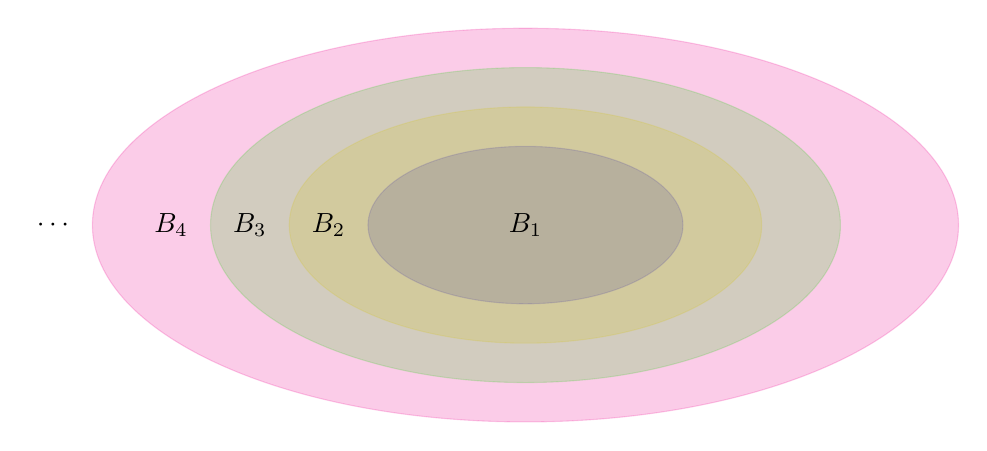
\begin{tikzpicture}
\draw[blue, fill, opacity=0.2] (0,0) ellipse [x radius=2cm, y radius=1cm];
\draw[yellow, fill, opacity=0.2] (0,0) ellipse [x radius=3cm, y radius=1.5cm];
\draw[green, fill, opacity=0.2] (0,0) ellipse [x radius=4cm, y radius=2cm];
\draw[magenta, fill, opacity=0.2] (0,0) ellipse [x radius=5.5cm, y radius=2.5cm];
\node[] () at (0,0) {\(B_1\)};
\node[] () at (-2.5,0) {\(B_2\)};
\node[] () at (-3.5,0) {\(B_3\)};
\node[] () at (-4.5,0) {\(B_4\)};
\node[] () at (-6,0) {\(\cdots\)};
\end{tikzpicture}
\end{center}
\item \underline{(1'), (2'), (3') \(\implies\) (1), (2), (3)}: 

Firstly, we have \(\varnothing=\Omega\setminus \Omega\in\mathcal{D}\) by (1')
and (2'). This shows (1).

For any \(A\in\mathcal{D}\), we have \(A^c=\Omega\setminus A\overset{\text{(2')}}{\in}\mathcal{D}\) as
\(A\subseteq \Omega\). This shows (2).

\textbf{Claim:} \(A_1,A_2\in\mathcal{D}\text{ pairwise disjoint}\implies
A_1\uplus A_2\in\mathcal{D}\).

\begin{pf}
Since \(A_1\cap A_2=\varnothing\), we have \(\brc{A_2}\subseteq
\vc{\Omega\setminus A_1}\).  By (1') and (2'), we know \(\vc{\Omega\setminus
A_1}\in\mathcal{D}\). Hence, by (2') again, we have \((\vc{\Omega\setminus
A_1})\setminus \brc{A_2}=\mgc{\Omega\setminus (A_1\uplus A_2)}\in\mathcal{D}\).
Using (2') once more, this implies \(A_1\uplus A_2=\Omega\setminus
(\mgc{\Omega\setminus (A_1\uplus A_2)})\in\mathcal{D}\).
\end{pf}

Fix any \(A_1,A_2,\dotsc\in\mathcal{D}\) that are pairwise disjoint. Let
\(B_n:=\biguplus_{i=1}^{n}A_i\) for every \(n\in\N\). Then
\(B_n\in\mathcal{D}\) by the claim and induction, and \(B_n\nearrow\). Thus
\(\biguplus_{n=1}^{\infty}A_n=\lim_{N\to \infty}\biguplus_{n=1}^{N}A_n
=\lim_{N\to \infty}\bigcup_{n=1}^{N}B_n =\bigcup_{n=1}^{\infty}B_n
\overset{\text{(3')}}{\in}\mathcal{D}\).
\end{itemize}
\item \textbf{Inclusion:} Fix any \(\sigma\)-algebra \(\mathcal{A}\) and any
\(A_1,A_2,\dotsc\in\mathcal{A}\) that are pairwise disjoint. Applying the
closedness under countable unions for \(\sigma\)-algebra, we have
\(\biguplus_{i=1}^{\infty}A_i\in\mathcal{A}\).

\textbf{Strictness:} Take \(\Omega=\{0,1,2,3\}\), \(A=\{0,1\}\), and
\(B=\{1,2\}\). Then the family \(\mathcal{D}=\{\varnothing,A,B,A^c,B^c,\Omega\}\)
is a Dynkin system (note that \(A\) and \(B\) are not pairwise disjoint), but
is not a \(\sigma\)-algebra since \(A\cup B=\{0,1,2\}\notin \mathcal{D}\).

\item Fix any \(A_1,A_2,\dotsc\in\mathcal{D}\). Let \(B_1:=A_1\in\mathcal{D}\)
and, for all \(n=2,3,\dotsc\), \(B_n:=A_n\setminus
\bigcup_{i=1}^{n-1}A_i=A_n\cap(\bigcup_{i=1}^{n-1}A_i)^{c}
\overset{\text{DM}}{=}A_n\cap\bigcap_{i=1}^{n-1}A_i^c \overset{\text{(2),
\(\pi\)-system}}{\in}\mathcal{D}\). Note that \(B_n\)'s are pairwise disjoint
and \(\bigcup_{n=1}^{N}A_n=\biguplus_{n=1}^{N}B_n\) for all \(N\in\N\).  Hence,
\[
\bigcup_{n=1}^{\infty}A_i=\lim_{N\to\infty}\bigcup_{n=1}^{N}A_n
=\lim_{N\to\infty}\biguplus_{n=1}^{N}B_n
=\biguplus_{n=1}^{\infty}B_n
\overset{\text{(3)}}{\in}\mathcal{D},
\]
thus \(\mathcal{D}\) is a \(\sigma\)-algebra.
\end{enumerate}
\end{pf}

\begin{note}
In the part (c) of the proof, the technique of constructing such pairwise
disjoint \(B_n\)'s out of general \(A_1,A_2,\dotsc\) is known as the
\defn{disjointification}, which is an useful tactic for measure theoretic
proof.
\end{note}

Because every \(\sigma\)-algebra is a Dynkin system, we indeed already know
many examples of Dynkin system.
\item \textbf{Dynkin systems generated by families of sets.}
Like \(\sigma\)-algebra, given a family \(\mathcal{A}\) of subsets of
\(\Omega\) and letting
\(\mathcal{D}_{\mathcal{A}}=\{\mathcal{D}:\text{\(\mathcal{D}\) is a Dynkin
system on \(\Omega\), \(\mathcal{D}\supseteq \mathcal{A}\)}\} \), the
\defn{Dynkin system generated by \(\mathcal{A}\)} is defined by
\(\defn{\text{\(\delta(\mathcal{A})\)}}:=\bigcap_{\mathcal{D}\in\mathcal{D}_{\mathcal{A}}}^{}\mathcal{D}\).


\textbf{Interpretation.} The family \(\delta(\mathcal{A})\) carries a similar
interpretation as before: \(\delta(\mathcal{A})\) is the smallest Dynkin system
on \(\Omega\) containing \(\mathcal{A}\),  i.e., (i) \(\delta(\mathcal{A})\) is
a Dynkin system on \(\Omega\) that contains \(\mathcal{A}\), and (ii) for all
Dynkin system \(\mathcal{D}'\) on \(\Omega\) with \(\vc{\mathcal{A}}\subseteq
\mathcal{D}'\), we have \(\delta(\vc{\mathcal{A}})\subseteq \mathcal{D}'\).

\begin{pf}
Analogous to the proof in \labelcref{it:sigma-alg-gen-interpret}.
\end{pf}

\item \textbf{Relationship between \(\delta(\mathcal{A})\) and
\(\sigma(\mathcal{A})\).} The two families \(\delta(\mathcal{A})\) and
\(\sigma(\mathcal{A})\) can be related by the following important theorem,
which gives us a sufficient condition for them to be equal.
\begin{theorem}[Dynkin's \(\pi\)-\(\lambda\) theorem]
\label{thm:dynkin-pi-lambda}
If \(\mathcal{D}\subseteq \mathcal{P}(\Omega)\) is a Dynkin system containing a
\emph{\(\pi\)-system} \(\mathcal{A}\), then (i) \(\sigma(\mathcal{A})\subseteq
\mathcal{D}\), which particularly implies (ii)
\(\delta(\mathcal{A})=\sigma(\mathcal{A})\).
\end{theorem}
An important strategy used in the proof is called the \emph{principle of good
sets}. It is also used in proving some other important theorems in measure
theory. This principle is usually utilized for showing that a certain property
holds for all elements of a \(\sigma\)-algebra \(\mathcal{F}\).

\textbf{\defn{Principle of good sets}.} Let \(\mathcal{G}\) be the family of
all ``good'' sets in \(\mathcal{F}\), which can be written as
\(\mathcal{G}=\{A\in\mathcal{F}:A\text{ satisfies a certain property}\}\). If
\(\mathcal{G}\) is a \underline{\(\sigma\)-algebra} that \underline{contains a
generator \(\vc{\mathcal{A}}\) for \(\mathcal{F}\)}, then we have
\(\mathcal{F}=\mathcal{G}\), meaning that \underline{every set in
\(\mathcal{F}\) is ``good''}.
\begin{note}
This is because we have \(\mathcal{F}=\sigma(\vc{\mathcal{A}})\subseteq
\mathcal{G}\), and \(\mathcal{G}\subseteq \mathcal{F}\) by construction.
\end{note}

\begin{remark}
\item The principle of good sets can be adapted for the case where \(\mathcal{F}\) is
a Dynkin system instead, by changing
\(\text{``\(\sigma\)-algebra''}\to\text{``Dynkin system''}\) and \(\sigma(\mathcal{A})\to\delta(\mathcal{A})\).
Such adapted version is used in the proof here.
\item After establishing the Dynkin's \(\pi\)-\(\lambda\) theorem below, due to
(i) in the theorem, we can apply the principle of good sets by showing
\(\mathcal{G}\) is a \underline{Dynkin system} that \underline{contains a
\(\pi\)-system \(\mathcal{A}\)} instead, but we would only be able to deduce
that every set in \(\sigma(\mathcal{A})\) (not necessarily \(\mathcal{F}\) in
this case) is ``good''.
\end{remark}

\begin{pf}
We first prove (i).

\textbf{Defining ``good''.} Fix any \(B\in\delta(\mathcal{A})\). We call a set
\(A\in\delta(\mathcal{A})\) ``good'' if it is still in \(\delta(\mathcal{A})\)
after intersecting with \(B\). \begin{intuition}
It is related with the closedness under intersections for a \(\pi\)-system.
\end{intuition}
Then, the family of all ``good'' sets in \(\delta(\mathcal{A})\) is
\[
\mathcal{D}_{B}:=\{A\in\delta(\mathcal{A}):A\cap B\in\delta(\mathcal{A})\}.
\]
\textbf{Showing that \(\mathcal{D}_{B}\) is a Dynkin system.}
\begin{enumerate}[label={(\arabic*)}]
\item Since \(\varnothing\in\delta(\mathcal{A})\) and \(\varnothing\cap
B=\varnothing\in\delta(\mathcal{A})\), we have \(\varnothing\in\mathcal{D}_{B}\).
\item Fix any \(A\in\mathcal{D}_{B}\). Then \(A\in\delta(\mathcal{A})\) and
\(A\cap B\in\delta(\mathcal{A})\). Thus \(\vc{A^c}\in\delta(\mathcal{A})\) and
\(\vc{A^c}\cap B=B\setminus (A\cap B)\overset{\text{(2')}}{\in}\delta(\mathcal{A})\) as \(A\cap B\subseteq B\).
Hence \(A^c\in\mathcal{D}_{B}\).
\item Fix any \(A_1,A_2,\dotsc\in\mathcal{D}_{B}\) that are pairwise disjoint.
Then for each \(i\in\N\), \(A_i\in\delta(\mathcal{A})\) and \(A_i\cap B\in\delta(\mathcal{A})\).
By closedness under countable disjoint unions for \(\delta(\mathcal{A})\), we have
\(\vc{\biguplus_{i=1}^{\infty}A_i}\in\delta(\mathcal{A})\). Also,
\((\vc{\biguplus_{i=1}^{\infty}A_i})\cap B
=\biguplus_{i=1}^{\infty}\underbrace{(A_i\cap B)}_{\in\delta(\mathcal{A})}
\in \delta(\mathcal{A})\). Thus \(\vc{\biguplus_{i=1}^{\infty}A_i}\in\mathcal{D}_{B}\).
\end{enumerate}
\textbf{Showing that \(\mathcal{D}_{B}\) contains a generator \(\mathcal{A}\) for the Dynkin system \(\delta(\mathcal{A})\).}

\textbf{Lemma:} For any \(A'\in\delta(\mathcal{A})\) and \(B'\in\mathcal{A}\), we have
\(A'\cap B'\in\delta(\mathcal{A})\).

\begin{pf}
Fix any \(B'\in\mathcal{A}\). Then for all \(\blc{A}\in\mathcal{A}\), since
\(\mathcal{A}\) is a \(\pi\)-system, we have \(\vc{A}\cap
B\in\mathcal{A}\subseteq \delta(\mathcal{A})\), which means
\(\blc{A}\in\mathcal{D}_{B'}\). Thus, \(\vc{\mathcal{A}}\subseteq
\mathcal{D}_{B'}\), which implies \(\delta(\vc{\mathcal{A}})\subseteq
\mathcal{D}_{B'}\) as \(\mathcal{D}_{B'}\) is a Dynkin system.

Having the inclusion \(\delta(\mathcal{A})\subseteq \mathcal{D}_{B'}\;\forall
B'\in\mathcal{A}\), we know that for all \(A'\in\delta(\mathcal{A})\) and
\(B'\in\mathcal{A}\), we have \(A'\in\mathcal{D}_{B'}\), so \(A'\cap
B'\in\delta(\mathcal{A})\).
\end{pf}

With the fixed \(B\in\delta(\mathcal{A})\), we want to show that
\(\mathcal{A}\subseteq \mathcal{D}_{B}\).  By the lemma with \(A'=B\) and
\(B'=A\), for all \(A\in\mathcal{A}\subseteq \delta(\mathcal{A})\), we have \(A\cap B\in\delta(\mathcal{A})\),
which means \(A\in\mathcal{D}_{B}\). Thus, \(\mathcal{A}\subseteq
\mathcal{D}_{B}\) as desired.

\textbf{Applying the principle of good sets to show that
\(\delta(\mathcal{A})\) is a \(\pi\)-system.} By the principle of good sets,
every set \(A\) in \(\delta(\mathcal{A})\) is ``good'', i.e, \(A\cap
B\in\delta(\mathcal{A})\), given any fixed \(B\in\delta(\mathcal{A})\). As this
holds for all \(B\in\delta(\mathcal{A})\), we know that
\(A,B\in\delta(\mathcal{A})\implies A\cap B\in\delta(\mathcal{A})\), implying
that \(\delta(\mathcal{A})\) is a \(\pi\)-system.

\textbf{Proving (i).} Since \(\delta(\mathcal{A})\) is a Dynkin system that is
also a \(\pi\)-system, \(\delta(\mathcal{A})\) is a \(\sigma\)-algebra
(containing \(\mathcal{A}\)). This shows \(\sigma(\mathcal{A})\subseteq
\delta(\mathcal{A})\). Also, since \(\mathcal{D}\) is a Dynkin system
containing \(\mathcal{A}\), we have \(\delta(\mathcal{A})\subseteq
\mathcal{D}\). Hence, \(\sigma(\mathcal{A})\subseteq \mathcal{D}\).

Next, we use (i) to prove (ii).  Firstly, (i) implies that
\(\sigma(\mathcal{A})\subseteq \delta(\mathcal{A})\) as \(\delta(\mathcal{A})\)
is a Dynkin system containing \(\mathcal{A}\). Also, since every
\(\sigma\)-algebra is a Dynkin system, \(\sigma(\mathcal{A})\) is a Dynkin
system containing \(\vc{\mathcal{A}}\), thus \(\delta(\vc{\mathcal{A}})\subseteq
\sigma(\mathcal{A})\). This completes the proof.
\end{pf}
\item \textbf{Borel \(\sigma\)-algebra.} Borel \(\sigma\)-algebra is a
\(\sigma\)-algebra generated by \emph{topology}, which is a family of open
sets. Before giving the formal definition, let us introduce/review what a
topology is. A \defn{topology} on a set \(\Omega\) is a family of subsets
\(\mathcal{T}\subseteq \mathcal{P}(\Omega)\) such that:
\begin{enumerate}[label={(\arabic*)}]
\item \(\varnothing,\Omega\in\mathcal{T}\).
\item \emph{(closed under arbitrary unions)} \(A_i\in\mathcal{T}\;\forall i\in I\implies \bigcup_{i\in I}^{}A_i\in\mathcal{T}\).
\item \emph{(closed under finite intersections)} \(A_1,\dotsc,A_n\in\mathcal{T}\implies \bigcap_{i=1}^{n}A_i\in\mathcal{T}\).
\end{enumerate}
\begin{intuition}
The closedness under arbitrary unions and finite intersections originate from
the property of openness and closedness for a \emph{metric space}: arbitrary
union of open sets is open, and finite intersection of open sets is open.
\end{intuition}

The pair \((\Omega,\mathcal{T})\) is called a \defn{topological space}. Every
set in \(\mathcal{T}\) is said to be \defn{open} in \(\Omega\), and the
complement of an open set in \(\Omega\) is said to be \defn{closed} in
\(\Omega\).\footnote{When we talk about a set is open/closed in \(\Omega\), such
set is understood to be a subset of \(\Omega\).}
\begin{note}
From this, we can see that the concepts of openness and closedness
are \emph{relative to} the topology \(\mathcal{T}\).
\end{note}

By default, when we talk about the case where \(\Omega=\R^d\), the
corresponding topology \(\mathcal{T}\) is supposed to be the ``usual
topology'', i.e., the one that is induced by the Euclidean metric, under which
our usual notion of ``open set'' and ``closed set'' (the concepts for
\emph{metric space}; see e.g., MATH3401) agrees with the openness and closedness
under the ``usual topology''. In general, a metric space can always induce a
corresponding topological space. (But we will mostly focus on the case
where \(\Omega=\R^d\) when discussing Borel \(\sigma\)-algebra.)

Let \((\Omega,\mathcal{T})\) be a topological space. Then the \defn{Borel
\(\sigma\)-algebra} on \(\Omega\) is given by
\(\defn{\text{\(\mathcal{B}(\Omega)\)}}:=\sigma(\mathcal{T})=\sigma(\{O:\text{\(O\)
is open in \(\Omega\)}\}\).  Every set in \(\mathcal{B}(\Omega)\) is called a
\defn{Borel set}.

From this definition, we can see that Borel \(\sigma\)-algebra is a rather
large family as it contains all open sets, closed sets, and countable
unions/intersections of these.
\item \textbf{Generators of Borel \(\sigma\)-algebras.} While Borel
\(\sigma\)-algebra is generated by all open sets, it may be a bit difficult to
understand intuitively what the generating process looks like. Fortunately, in
the special case where \(\Omega=\R\) or \(\Omega=\R^d\), some alternative
and perhaps more intuitive generators are available.

First we consider the case where \(\Omega=\R\). To derive an alternative
generator, we need the following lemma.
\begin{lemma}
\label{lma:open-set-r-open-int}
Every open set in \(\R\) is a countable disjoint union of open intervals.
\end{lemma}
\begin{pf}
Fix any open \(O\subseteq \R\). For any \(x\in O\), let
\(\mathcal{J}_x:=\{I:\text{\(I\) is an open interval in \(O\) and \(x\in
I\)}\}\) and \(I_x:=\bigcup_{I\in\mathcal{J}_x}^{}I\) be the open interval of
maximal length containing \(x\) (in \(O\)).
\begin{center}
\begin{tikzpicture}
\draw[-Latex] (0,0) -- (10,0);
\draw[blue, fill] (5,0) circle [radius=0.5mm];
\node[] () at (5,0.3) {\(x\)};
\node[violet] () at (3,0) {(};
\node[violet] () at (8,0) {)};
\node[magenta] () at (2,0) {(};
\node[magenta] () at (6,0) {)};
\node[orange] () at (3.5,0) {(};
\node[orange] () at (7,0) {)};
\end{tikzpicture}
\end{center}
If \(x,y\in O\), then we have either \(I_x=I_y\) or \(I_x\cap I_y=\varnothing\)
by construction. By the axiom of choice, we select \(I_x\) for every \(x\in
O\). Collecting them with redundancies removed, we get a set
\(\mathcal{I}=\{I_x:x\in O\}\) of all distinct and pairwise disjoint intervals
of maximal length.

Then, we have \(O=\bigcup_{x\in O}^{}I_x=\biguplus_{I\in\mathcal{I}}^{}I\).
The latter disjoint union is countable since we can define an injection \(f\)
from \(\mathcal{I}\) to \(\Q\) (countable) by \(f(I)=q_I\in\Q\) where \(q_I\)
is any rational number in \(I\) (which exists due to the density of \(\Q\) on
\(\R\)). (The injectivity follows from the pairwise disjointness of intervals
in \(\mathcal{I}\).)
\end{pf}

Having \Cref{lma:open-set-r-open-int}, we can derive another generator for
Borel \(\sigma\)-algebra on \(\R\), which is the family of all \emph{open
intervals}. It turns out that, while the family of all open intervals appears
to be much smaller than the family \(\mathcal{T}\) of all open sets in \(\R\),
it can still generate the Borel \(\sigma\)-algebra!

\begin{proposition}[\(\mathcal{B}(\R)\) is generated by all open intervals]
\label{prp:borel-r-gen-by-open-int}
We have \(\mathcal{B}(\R)=\sigma(\{(a,b):a<b\})\).
\end{proposition}
\begin{note}
Sometimes the shorthand notation \(\mathcal{B}\) is used instead of \(\mathcal{B}(\R)\).
\end{note}

\begin{pf}
``\(\supseteq\)'': Note that \(\vc{\{(a,b):a<b\}}\subseteq \{O:\text{\(O\) open
in \(\R\)}\}=\mathcal{T}\subseteq \sigma(\mathcal{T})=\mathcal{B}(\R)\). Thus,
by the minimality we have
\(\sigma(\vc{\{(a,b):a<b\}})\subseteq\mathcal{B}(\R)\).

``\(\subseteq\)'': By \Cref{lma:open-set-r-open-int}, every open \(O\subseteq
\R\) is a countable disjoint union of open intervals, hence is in
\(\sigma(\{(a,b):a<b\})\).  It follows that \(\vc{\mathcal{T}}=\{O:\text{\(O\)
is open in \(\R\)}\}\subseteq\sigma(\{(a,b):a<b\})\), thus
\(\mathcal{B}(\R)=\sigma(\vc{\mathcal{T}})\subseteq \sigma(\{(a,b):a<b\})\) by
the minimality.
\end{pf}

More generally, we have the following result.
\begin{proposition}[Generators of \(\mathcal{B}(\R^d)\)]
\label{prp:borel-rd-generators}
We have
\begin{align*}
\mathcal{B}(\R^d)
&=\sigma(\{(\vect{a},\vect{b}):\vect{a},\vect{b}\in\R^d, \vect{a}<\vect{b}\})
=\sigma(\{[\vect{a},\vect{b}]:\vect{a},\vect{b}\in\R^d, \vect{a}<\vect{b}\}) \\
&=\sigma(\{(\vect{a},\vect{b}]:\vect{a},\vect{b}\in\R^d, \vect{a}<\vect{b}\})
=\sigma(\{[\vect{a},\vect{b}):\vect{a},\vect{b}\in\R^d, \vect{a}<\vect{b}\}) \\
&=\sigma(\{(\vect{-\infty},\vect{b}):\vect{b}\in\R^d\})
=\sigma(\{(\vect{a},\vect{\infty}):\vect{a}\in\R^d\}) \\
&=\sigma(\{(\vect{-\infty},\vect{b}]:\vect{b}\in\R^d\})
=\sigma(\{[\vect{a},\vect{\infty}):\vect{a}\in\R^d\}).
\end{align*}
\end{proposition}
\begin{note}
Here, the interval and inequality notations carry componentwise meaning:
\(\vect{a}<\vect{b}\) means \(a_i<b_i\) for all \(i=1,\dotsc,d\),
\((\vect{a},\vect{b})=(a_1,b_1)\times\dotsb\times (a_d,b_d)\), etc., where
\(\vect{a}=(a_1,\dotsc,a_d)\) and \(\vect{b}=(b_1,\dotsc,b_d)\).
\end{note}
\begin{pf}
Omitted.
\end{pf}
\item \textbf{Borel \(\sigma\)-algebras on \(\R^d\), \(\eR{}^d\), and their subsets.}
\begin{enumerate}
\item\label{it:borel-rd-prod-sig} The Borel \(\sigma\)-algebra \(\mathcal{B}(\R^d)\) is the
product \(\sigma\)-algebra \(\bigotimes_{i=1}^{d}\mathcal{B}(\R)\).
\item Later in \Cref{sect:integration-expectation}, we will encounter the case
\(\Omega=\eR:=\R\cup\{-\infty,\infty\}=:[-\infty,\infty]\), the extended real
number system. An order topology can be equipped on \(\eR\) to form a
topological space. Then it can be shown that \(A\subseteq \eR\) is open iff
\(A\) is a countable union of members in
\(\{(a,b):a,b\in\R\}\cup\{[-\infty,b):b\in\R\}\cup\{(a,\infty]:a\in\R\}\).

Consequently, we have \(\mathcal{B}(\eR)=\{B\cup E:B\in\mathcal{B}(\R), E\subseteq \{-\infty,\infty\}\}\).
From this we can get, e.g., \(\mathcal{B}(\eR)=\sigma(\{(a,\infty]:a\in\R\})
\) and \(\mathcal{B}(\eR)=\sigma(\{[-\infty,b]:b\in\R\})\).

\item The Borel \(\sigma\)-algebra \(\mathcal{B}(\eR{}^d)\) is the
product \(\sigma\)-algebra \(\bigotimes_{i=1}^{d}\mathcal{B}(\eR)\).

\item Borel \(\sigma\)-algebra on \(\Omega\subseteq \R^d\) or \(\Omega\subseteq
\eR{}^d\) can be obtained by the respective \emph{trace \(\sigma\)-algebra}.
For instance, if \(\Omega\subseteq \R^d\), then
\(\mathcal{B}(\Omega)=\mathcal{B}(\R^d)|_{\Omega}
=\{B\cap\Omega:B\in\mathcal{B}(\R^d)\}\).

\end{enumerate}
\end{enumerate}
